\renewcommand{\thesection}{\Alph{section}}%
\appendix 
\addcontentsline{toc}{chapter}{Anhang} 

%%%%%%%%%%%%%%%%%%%%%%%%
%%%%%%%%%%%%%%%%%%%%%%%%
%%%%%%%%%%%%%%%%%%%%%%%%

\section{Studie zu Affixen}
\label{affix_studie}
Zur Identifizierung möglichst vieler relevanter Prä- und Suffixe habe ich eine kleine Studie zu betonten/unbetonten Affixen durchgeführt. Hierfür habe ich einen Entscheidungsbaum mittels REPTree aus WEKA auf dem kompletten Datensatz (ohne Komposita) je Silbe trainiert. Als Features dienten mir lediglich die Suffixe bzw. Präfixe.  
Ich habe deutlich mehr Suffixe als Präfixe gefunden, die eine eindeutige Betonungsklasse identifizieren. Aus allen Affixen habe ich die mit weniger als 10\% Ausnahmen identifiziert.
Datensätze mit wenigen Silben haben mehr eindeutig betonte oder unbetonte Affixe. Bemerkenswert ist, dass es bei den Wörtern mit mehr als 3 Silben kein signifikantes Affix gibt, dass sich nicht schon bei den Zwei- und Dreisilbern als wichtig herausgestellt hat. Man kann jedoch bei einigen Affixen feststellen, dass sie häufiger eindeutig betont/unbetont sind als andere, beispielsweise -ik und -ismus. Ich vermute dass bei kurzen Wörtern es weniger andere Phänomene auftreten können, als bei langen Wörtern. Dies wäre ein Indiz für die sogenannte XYZ Hypothese, wie sie unter anderem in [CITE] formuliert wurde. Darüber hinausgehend formuliere ich die Hypothese, dass es nicht nur betonte und unbetonte Affixe gibt wie in [CITE] angegeben, sondern verschiedene Grade an Anzieungskraft der Betonung gibt. Ausgehend von der Hypothese, dass mehrere Betonungsregeln in wechselseitiger Beziehung zu einer stehen erscheint es um so sinnvoller neben Entscheidungsbäumen und Propositional Rule Learnern auch nichtlineare Neuronale Netze in die Untersuchung mit einzubeziehn, die im gegensatz zu den beiden erstgenannten Verfahren diese interdependeznen abbilden können.
\begin{table}[h]
\centering
\caption{Betonte Präfixe in Nonkomposita}
\resizebox{\columnwidth}{!}{%
\begin{tabular}{|l|lllllllllllllllllllllll|}
\hline
{\bf Silben} & \multicolumn{23}{c|}{{\bf Betontes Präfixe}} \\ \hline
2	& ab	& ~	& auf	& aus	& bei	& durch	& ein	& fern	& fort	& gegen	& hinter	& hin	& hoch	& mit	& nach	& ueber	& um	& unter	& ur	& vor	& weg	& ~	& \\ 
3	& ab	& an	& auf	& aus	& ~	& ~	& ein	& fern	& fort	& gegen	& hinter	& hin	& hoch	& mit	& nach	& ueber	& ~	& unter	& ur	& vor	& weg	& zu\\ 
4	& ab	& an	& auf	& aus	& ~	& durch	& ein	& fern	& fort	& ~	& ~	& ~	& ~	& mit	& nach	& ~	& ~	& ~	& ur	& ~	& 	& ~	& \\ 
5	& ~	& an	& auf	& aus	& ~	& ~	& ein	& ~	& ~	& gegen	& hinter	& ~	& hoch	& mit	& ~	& ~	& um	& ~	& ur	& ~	& 	& ~	& \\ 
6	& ab	& ~	& auf	& aus	& ~	& ~	& ~	& ~	& ~	& ~	& ~	& ~	& ~	& ~	& ~	& ueber	& um	& unter	& ~	& 	& ~	& \\  \hline
$\Rightarrow$	& ab	& an	& auf	& aus	& bei	& durch	& ein	& fern	& fort	& gegen	& hinter	& hin	& hoch	& mit	& nach	& ueber	& um	& unter	& ur	& vor	& weg	& zu \\ \hline
\end{tabular}%
}
\end{table}
\begin{table}[h]
\centering
\small
\caption{Unbetonte Suffixe in Nonkomposita}
\resizebox{\columnwidth}{!}{%
\begin{tabular}{|l|llllllllllllllll|}
\hline
{\bf Silben}     & \multicolumn{16}{c|}{{\bf Betontes Suffixe}} \\ \hline
2                & ig &  ik  &         &  bar    & er   & sam & ung & isch & lich & heit & ler   & ling & schaft & nis    & tum  & ~     \\
3                & ig &  ik  &   ismus &  ~      & ~    &    ~&  ~   &   ~ &     ~ &  ~   &    ~ & ling & ~      &  nis   & tum  & keit  \\
4                & ~  &  ik  &   ismus &  ~      & ~    &    ~&  ~   &   ~ &     ~ &  ~   &  ~   &  ~   & ~      &    ~   & ~    & ~     \\
5                &    &  ik  &   ismus &  ~      & ~    &    ~&   ~  &   ~ &  ~    & ~    &  ~   & ~    &    ~   &  ~     & tum  & ~     \\
6                & ig &  ik  &   ismus &  ~      & ~    &    ~&   ~  &   ~ & lich  & ~    &  ler & ~    &  ~     & ~      & tum  & ~     \\ \hline
$\Rightarrow$    & ig &  ik  &   ismus &  ~	     & ~	&    ~&   ~  &   ~ & lich  & ~    & ler  & ling & ~      &  nis   & tum  & keit  \\ \hline
\end{tabular}%
}
\end{table}
\begin{table}[h]
\centering
\caption{Unbetonte Präfixe in Nonkomposita}
\begin{tabular}{|l|lllll|}
\hline
{\bf Silben}       & \multicolumn{5}{c|}{{\bf Unbetontes Suffixe}} \\ \hline
2                  & be-     & ent-   & er-   & ver-   & zer-   \\
3                  & be-     & ent-   & er-   & ver-   & zer-   \\
4                  & be-     & ent-   & er-   & ver-   & zer-   \\
5                  & be-     &        & er-   & ver-   &        \\
6                  & be-     &        & er-   &        &        \\ \hline
{\bf Als Feature:} & be-     & ent-   & er-   & ver-   & zer-  \\ \hline
\end{tabular}
\end{table}
\begin{table}[h]
\centering
\caption{Betonte Suffixe bei Nonkomposita}
\begin{tabular}{|l|cc|}
\hline
{\bf Silben}       & \multicolumn{2}{c|}{{\bf Betontes Suffixe}} \\ \hline
2                  &                      &                     \\
3                  & -ist                 & -ei                 \\
4                  & -ist                 & -ei                 \\
5                  & -ist                 & -ei                 \\
6                  & -ist                 &                     \\ \hline
{\bf Als Feature:} & -ist                 & -ei                 \\ \hline
\end{tabular}
\end{table}


%%%%%%%%%%%%%%%%%%%%%%%%

\section{Features und Featuresets}
\label{detail_performance}
Die Summen am Ende der Tabelle beziehen sich auf die Anzahl der Werte aller Features eines Featuresets. Numerische Attribute Zählen als $1$. So gesehen ist die entsprechende Summe gleich der Anzahl an Neuronen im Input-Layer des Neuronalen Netzes.
\footnotesize
\begin{longtable}{|r|llllll|c|}

    \caption{Anzahl Werte je Attribut}
    \label{table:feature_dimensions}\\
    
    \hline
    \diagbox{{\bf Attribut}}{{\bf Silben}} & 2 & 3 & 4 & 5 & 6 & 7 & Erwartungswert \\ \hline
    syl\_suffix       & 54   & 94   & 65   & 22   & 5    & 2    & 68,4     \\
    signi\_suffix     & 23   & 37   & 29   & 20   & 13   & 9    & 29,4     \\
    suffix1           & 23   & 22   & 21   & 21   & 18   & 12   & 21,8     \\
    suffix2           & 71   & 71   & 47   & 22   & 9    & 2    & 59,5     \\
    suffix3           & 94   & 116  & 80   & 21   & 8    & 2    & 90,9     \\
    suffix4           & 42   & 115  & 60   & 17   & 8    & 2    & 72,1     \\
    suffix5           & 28   & 144  & 71   & 23   & 8    & 3    & 83,1     \\
    suffix\_phoncat1  & 6    & 6    & 6    & 6    & 5    & 5    & 6        \\
    suffix\_phoncat2  & 11   & 11   & 9    & 7    & 6    & 3    & 10       \\
    suffix\_phoncat3  & 21   & 25   & 19   & 12   & 7    & 2    & 20,9     \\
    suffix\_phoncat4  & 30   & 32   & 24   & 17   & 9    & 2    & 27,7     \\
    suffix\_phoncat5  & 31   & 45   & 36   & 22   & 6    & 2    & 36,3     \\
    suff\_class       & 3    & 3    & 3    & 3    & 3    & 3    & 3        \\
    syl\_praefix      & 45   & 102  & 94   & 37   & 4    & 1    & 77,3     \\
    signi\_praefix    & 23   & 24   & 22   & 20   & 14   & 5    & 22,6     \\
    praefix1          & 50   & 50   & 50   & 49   & 45   & 36   & 49,7     \\
    praefix2          & 107  & 130  & 86   & 25   & 2    & 1    & 101,4    \\
    praefix3          & 30   & 86   & 42   & 11   & 1    & 1    & 52,6     \\
    praefix4          & 26   & 106  & 37   & 7    & 1    & 1    & 58,1     \\
    praefix5          & 10   & 35   & 18   & 6    & 1    & 1    & 21,2     \\
    praefix\_phoncat1 & 6    & 6    & 6    & 5    & 5    & 5    & 5,9      \\
    praefix\_phoncat2 & 12   & 12   & 12   & 9    & 7    & 4    & 11,6     \\
    praefix\_phoncat3 & 24   & 29   & 28   & 17   & 8    & 4    & 25,9     \\
    praefix\_phoncat4 & 42   & 52   & 40   & 21   & 13   & 2    & 42,9     \\
    praefix\_phoncat5 & 52   & 76   & 52   & 27   & 11   & 1    & 58,2     \\
    prae\_class       & 3    & 3    & 3    & 3    & 3    & 3    & 3        \\
    sonority0         & 1    & 1    & 1    & 1    & 1    & 1    & 1        \\
    sonority1         & 1    & 1    & 1    & 1    & 1    & 1    & 1        \\
    sonority2         & ~    & 1    & 1    & 1    & 1    & 1    & 1        \\
    sonority3         & ~    & ~    & 1    & 1    & 1    & 1    & 1        \\
    sonority4         & ~    & ~    & ~    & 1    & 1    & 1    & 1        \\
    sonority5         & ~    & ~    & ~    & ~    & 1    & 1    & 1        \\
    sonority6         & ~    & ~    & ~    & ~    & ~    & 1    & 1        \\
    sonority\_ratio0  & 1    & 1    & 1    & 1    & 1    & 1    & 1        \\
    sonority\_ratio1  & 1    & 1    & 1    & 1    & 1    & 1    & 1        \\
    sonority\_ratio2  & ~    & 1    & 1    & 1    & 1    & 1    & 1        \\
    sonority\_ratio3  & ~    & ~    & 1    & 1    & 1    & 1    & 1        \\
    sonority\_ratio4  & ~    & ~    & ~    & 1    & 1    & 1    & 1        \\
    sonority\_ratio5  & ~    & ~    & ~    & ~    & 1    & 1    & 1        \\
    sonority\_ratio6  & ~    & ~    & ~    & ~    & ~    & 1    & 1        \\
    sonority\_dir     & 1    & 1    & 1    & 1    & 1    & 1    & 1        \\
    syl\_weight0      & 3    & 3    & 3    & 3    & 3    & 3    & 3        \\
    syl\_weight1      & 4    & 3    & 3    & 3    & 3    & 3    & 3,3      \\
    syl\_weight2      & ~    & 3    & 3    & 3    & 3    & 3    & 3        \\
    syl\_weight3      & ~    & ~    & 4    & 3    & 3    & 3    & 3,7      \\
    syl\_weight4      & ~    & ~    & ~    & 4    & 3    & 3    & 3,8      \\
    syl\_weight5      & ~    & ~    & ~    & ~    & 3    & 3    & 3        \\
    syl\_weight6      & ~    & ~    & ~    & ~    & ~    & 3    & 3        \\
    syl\_open0        & 2    & 2    & 2    & 2    & 2    & 2    & 2        \\
    syl\_open1        & 3    & 2    & 2    & 2    & 2    & 2    & 2,3      \\
    syl\_open2        & ~    & 2    & 2    & 2    & 2    & 2    & 2        \\
    syl\_open3        & ~    & ~    & 3    & 2    & 2    & 2    & 2,7      \\
    syl\_open4        & ~    & ~    & ~    & 3    & 2    & 2    & 2,8      \\
    syl\_open5        & ~    & ~    & ~    & ~    & 2    & 2    & 2        \\
    syl\_open6        & ~    & ~    & ~    & ~    & ~    & 2    & 2        \\
    syl\_phoncat0     & 37   & 40   & 30   & 18   & 8    & 5    & 34,1     \\
    syl\_phoncat1     & 33   & 36   & 26   & 17   & 9    & 4    & 30,5     \\
    syl\_phoncat2     & ~    & 32   & 30   & 18   & 10   & 4    & 28,9     \\
    syl\_phoncat3     & ~    & ~    & 22   & 16   & 11   & 5    & 19,6     \\
    syl\_phoncat4     & ~    & ~    & ~    & 14   & 7    & 3    & 12,1     \\
    syl\_phoncat5     & ~    & ~    & ~    & ~    & 8    & 5    & 7,4      \\
    syl\_phoncat6     & ~    & ~    & ~    & ~    & ~    & 5    & 5        \\
    onset\_phoncat0   & 6    & 5    & 6    & 5    & 4    & 4    & 5,5      \\
    onset\_phoncat1   & 7    & 5    & 5    & 5    & 5    & 3    & 5,5      \\
    onset\_phoncat2   & ~    & 5    & 6    & 6    & 4    & 3    & 5,4      \\
    onset\_phoncat3   & ~    & ~    & 6    & 5    & 3    & 3    & 5,5      \\
    onset\_phoncat4   & ~    & ~    & ~    & 6    & 5    & 4    & 5,7      \\
    onset\_phoncat5   & ~    & ~    & ~    & ~    & 3    & 3    & 3        \\
    onset\_phoncat6   & ~    & ~    & ~    & ~    & ~    & 2    & 2        \\
    koda\_phoncat0    & 8    & 8    & 7    & 6    & 6    & 3    & 7,5      \\
    koda\_phoncat1    & 9    & 7    & 6    & 5    & 4    & 3    & 7        \\
    koda\_phoncat2    & ~    & 7    & 7    & 4    & 5    & 3    & 6,6      \\
    koda\_phoncat3    & ~    & ~    & 8    & 4    & 4    & 3    & 6,7      \\
    koda\_phoncat4    & ~    & ~    & ~    & 7    & 3    & 3    & 6        \\
    koda\_phoncat5    & ~    & ~    & ~    & ~    & 5    & 2    & 4,4      \\
    koda\_phoncat6    & ~    & ~    & ~    & ~    & ~    & 3    & 3        \\
    nucleus\_phoncat0 & 4    & 4    & 4    & 4    & 3    & 3    & 4        \\
    nucleus\_phoncat1 & 5    & 4    & 4    & 4    & 4    & 3    & 4,3      \\
    nucleus\_phoncat2 & ~    & 4    & 4    & 4    & 3    & 3    & 4        \\
    nucleus\_phoncat3 & ~    & ~    & 5    & 4    & 4    & 3    & 4,7      \\
    nucleus\_phoncat4 & ~    & ~    & ~    & 5    & 3    & 3    & 4,5      \\
    nucleus\_phoncat5 & ~    & ~    & ~    & ~    & 3    & 3    & 3        \\
    nucleus\_phoncat6 & ~    & ~    & ~    & ~    & ~    & 4    & 4        \\
    syl\_len0         & 1    & 1    & 1    & 1    & 1    & 1    & 1        \\
    syl\_len1         & 1    & 1    & 1    & 1    & 1    & 1    & 1        \\
    syl\_len2         & ~    & 1    & 1    & 1    & 1    & 1    & 1        \\
    syl\_len3         & ~    & ~    & 1    & 1    & 1    & 1    & 1        \\
    syl\_len4         & ~    & ~    & ~    & 1    & 1    & 1    & 1        \\
    syl\_len5         & ~    & ~    & ~    & ~    & 1    & 1    & 1        \\
    syl\_len6         & ~    & ~    & ~    & ~    & ~    & 1    & 1        \\
    koda\_len0        & 1    & 1    & 1    & 1    & 1    & 1    & 1        \\
    koda\_len1        & 1    & 1    & 1    & 1    & 1    & 1    & 1        \\
    koda\_len2        & ~    & 1    & 1    & 1    & 1    & 1    & 1        \\
    koda\_len3        & ~    & ~    & 1    & 1    & 1    & 1    & 1        \\
    koda\_len4        & ~    & ~    & ~    & 1    & 1    & 1    & 1        \\
    koda\_len5        & ~    & ~    & ~    & ~    & 1    & 1    & 1        \\
    koda\_len6        & ~    & ~    & ~    & ~    & ~    & 1    & 1        \\
    onset\_len0       & 1    & 1    & 1    & 1    & 1    & 1    & 1        \\
    onset\_len1       & 1    & 1    & 1    & 1    & 1    & 1    & 1        \\
    onset\_len2       & ~    & 1    & 1    & 1    & 1    & 1    & 1        \\
    onset\_len3       & ~    & ~    & 1    & 1    & 1    & 1    & 1        \\
    onset\_len4       & ~    & ~    & ~    & 1    & 1    & 1    & 1        \\
    onset\_len5       & ~    & ~    & ~    & ~    & 1    & 1    & 1        \\
    onset\_len6       & ~    & ~    & ~    & ~    & ~    & 1    & 1        \\
    nucleus\_len0     & 1    & 1    & 1    & 1    & 1    & 1    & 1        \\
    nucleus\_len1     & 1    & 1    & 1    & 1    & 1    & 1    & 1        \\
    nucleus\_len2     & ~    & 1    & 1    & 1    & 1    & 1    & 1        \\
    nucleus\_len3     & ~    & ~    & 1    & 1    & 1    & 1    & 1        \\
    nucleus\_len4     & ~    & ~    & ~    & 1    & 1    & 1    & 1        \\
    nucleus\_len5     & ~    & ~    & ~    & ~    & 1    & 1    & 1        \\
    nucleus\_len6     & ~    & ~    & ~    & ~    & ~    & 1    & 1        \\
    syl\_cv0          & 19   & 19   & 17   & 13   & 8    & 4    & 17,7     \\
    syl\_cv1          & 17   & 19   & 15   & 11   & 9    & 3    & 16,6     \\
    syl\_cv2          & ~    & 18   & 17   & 12   & 8    & 3    & 16,6     \\
    syl\_cv3          & ~    & ~    & 15   & 10   & 8    & 3    & 13,1     \\
    syl\_cv4          & ~    & ~    & ~    & 10   & 6    & 3    & 8,9      \\
    syl\_cv5          & ~    & ~    & ~    & ~    & 8    & 3    & 7,1      \\
    syl\_cv6          & ~    & ~    & ~    & ~    & ~    & 7    & 7        \\
    cv\_ratio0        & 1    & 1    & 1    & 1    & 1    & 1    & 1        \\
    cv\_ratio1        & 1    & 1    & 1    & 1    & 1    & 1    & 1        \\
    cv\_ratio2        & ~    & 1    & 1    & 1    & 1    & 1    & 1        \\
    cv\_ratio3        & ~    & ~    & 1    & 1    & 1    & 1    & 1        \\
    cv\_ratio4        & ~    & ~    & ~    & 1    & 1    & 1    & 1        \\
    cv\_ratio5        & ~    & ~    & ~    & ~    & 1    & 1    & 1        \\
    cv\_ratio6        & ~    & ~    & ~    & ~    & ~    & 1    & 1        \\
    pos               & 5    & 5    & 5    & 5    & 4    & 4    & 5        \\
    comp\_struct      & 13   & 18   & 17   & 14   & 8    & 2    & 15,8     \\
    nomen             & 2    & 2    & 2    & 2    & 2    & 2    & 2        \\
    comp\_len         & 1    & 1    & 1    & 1    & 1    & 1    & 1        \\
    stress\_class     & 2    & 3    & 4    & 5    & 5    & 5    & 3,2      \\ \hline
    praefix           & 430  & 711  & 490  & 237  & 115  & 65   & 530,3    \\
    suffix            & 437  & 721  & 470  & 213  & 105  & 49   & 529,1    \\
    affix             & 867  & 1432 & 960  & 450  & 220  & 114  & 1059,4   \\
    phoncat           & 109  & 157  & 176  & 157  & 124  & 95   & 148,1    \\
    sonority          & 5    & 7    & 9    & 11   & 13   & 15   & 7,5      \\
    weight            & 12   & 15   & 22   & 27   & 30   & 35   & 17,3     \\
    phon              & 126  & 179  & 207  & 195  & 167  & 145  & 172,9    \\
    sylstruct         & 46   & 71   & 84   & 81   & 77   & 61   & 68,6     \\
    meta              & 21   & 26   & 25   & 22   & 15   & 9    & 23,8     \\
    sparse            & 80   & 100  & 133  & 151  & 157  & 162  & 108,5    \\
    numeric           & 16   & 23   & 30   & 37   & 44   & 51   & 24,6     \\
    all               & 1061 & 1710 & 1279 & 752  & 484  & 334  & 1326,9   \\ \hline
\end{longtable}
\normalsize
\ref{attr_counts}
\newpage

%\begin{landscape}

\clearpage
\label{featurematrix}
\begin{sidewaystable}
\section{Feautrematrix}
\centering
\resizebox{\columnwidth}{!}{%
\begin{tabular}{|l|l|l|l|l|l|l|l|l|l|l|l|l|}
\hline
{\bf }                    & {\bf praefix} & {\bf suffix} & {\bf affix} & {\bf phoncat} & {\bf weight} & {\bf sonority} & {\bf phon} & {\bf sylstruct} & {\bf meta} & {\bf sparse} & {\bf numeric} & {\bf all} \\ \hline
syl\_suffix               &               & X            & X           &               &              &                &            &                 &            &              &               & X         \\ \hline
signi\_suffix             &               & X            & X           &               &              &                &            &                 &            &              &               & X         \\ \hline
suffix{[}1-5{]}           &               & X            & X           &               &              &                &            &                 &            &              &               & X         \\ \hline
suffix\_phoncat{[}1-5{]}  &               & X            & X           &               &              &                &            &                 &            &              &               & X         \\ \hline
suff\_class               &               & X            & X           &               &              &                &            &                 &            & X            &               & X         \\ \hline
syl\_praefix              & X             &              & X           &               &              &                &            &                 &            &              &               & X         \\ \hline
signi\_praefix            & X             &              & X           &               &              &                &            &                 &            &              &               & X         \\ \hline
praefix{[}1-5{]}          & X             &              & X           &               &              &                &            &                 &            &              &               & X         \\ \hline
praefix\_phoncat{[}1-5{]} & X             &              & X           &               &              &                &            &                 &            &              &               & X         \\ \hline
prae\_class               & X             &              & X           &               &              &                &            &                 &            & X            &               & X         \\ \hline
sonority{[}i{]}           &               &              &             &               &              & X              & X          &                 &            & X            & X             & X         \\ \hline
sonority\_ratio{[}i{]}    &               &              &             &               &              & X              & X          &                 &            & X            & X             & X         \\ \hline
sonority\_dir             &               &              &             &               &              & X              & X          &                 &            & X            & X             & X         \\ \hline
syl\_weight{[}i{]}        &               &              &             &               & X            &                & X          &                 &            & X            &               & X         \\ \hline
syl\_open{[}i{]}          &               &              &             &               & X            &                & X          &                 &            & X            &               & X         \\ \hline
syl\_phoncat{[}i{]}       &               &              &             & X             &              &                & X          &                 &            &              &               & X         \\ \hline
onset\_phoncat{[}i{]}     &               &              &             & X             &              &                & X          &                 &            & X            &               & X         \\ \hline
koda\_phoncat{[}i{]}      &               &              &             & X             &              &                & X          &                 &            & X            &               & X         \\ \hline
nucleus\_phoncat{[}i{]}   &               &              &             & X             &              &                & X          &                 &            & X            &               & X         \\ \hline
syl\_len{[}i{]}           &               &              &             &               &              &                &            & X               &            & X            & X             & X         \\ \hline
koda\_len{[}i{]}          &               &              &             &               &              &                &            & X               &            & X            & X             & X         \\ \hline
onset\_len{[}i{]}         &               &              &             &               &              &                &            & X               &            & X            & X             & X         \\ \hline
nucleus\_len{[}i{]}       &               &              &             &               &              &                &            & X               &            & X            & X             & X         \\ \hline
syl\_cv{[}i{]}            &               &              &             &               &              &                &            & X               &            &              &               & X         \\ \hline
cv\_ratio{[}i{]}          &               &              &             &               &              &                &            & X               &            & X            & X             & X         \\ \hline
pos                       &               &              &             &               &              &                &            &                 & X          & X            &               & X         \\ \hline
comp\_struct              &               &              &             &               &              &                &            &                 & X          &              &               & X         \\ \hline
nomen                     &               &              &             &               &              &                &            &                 & X          & X            &               & X         \\ \hline
comp\_len                 &               &              &             &               &              &                &            &                 & X          & X            & X             & X         \\ \hline
\end{tabular}%
}
\caption{Featuresetmatrix}
\end{sidewaystable}
\clearpage
%\end{landscape}

%%%%%%%%%%%%%%%%%%%%

\section{Detailierte Erkennungsraten}
\label{performance_details}
\begin{center}{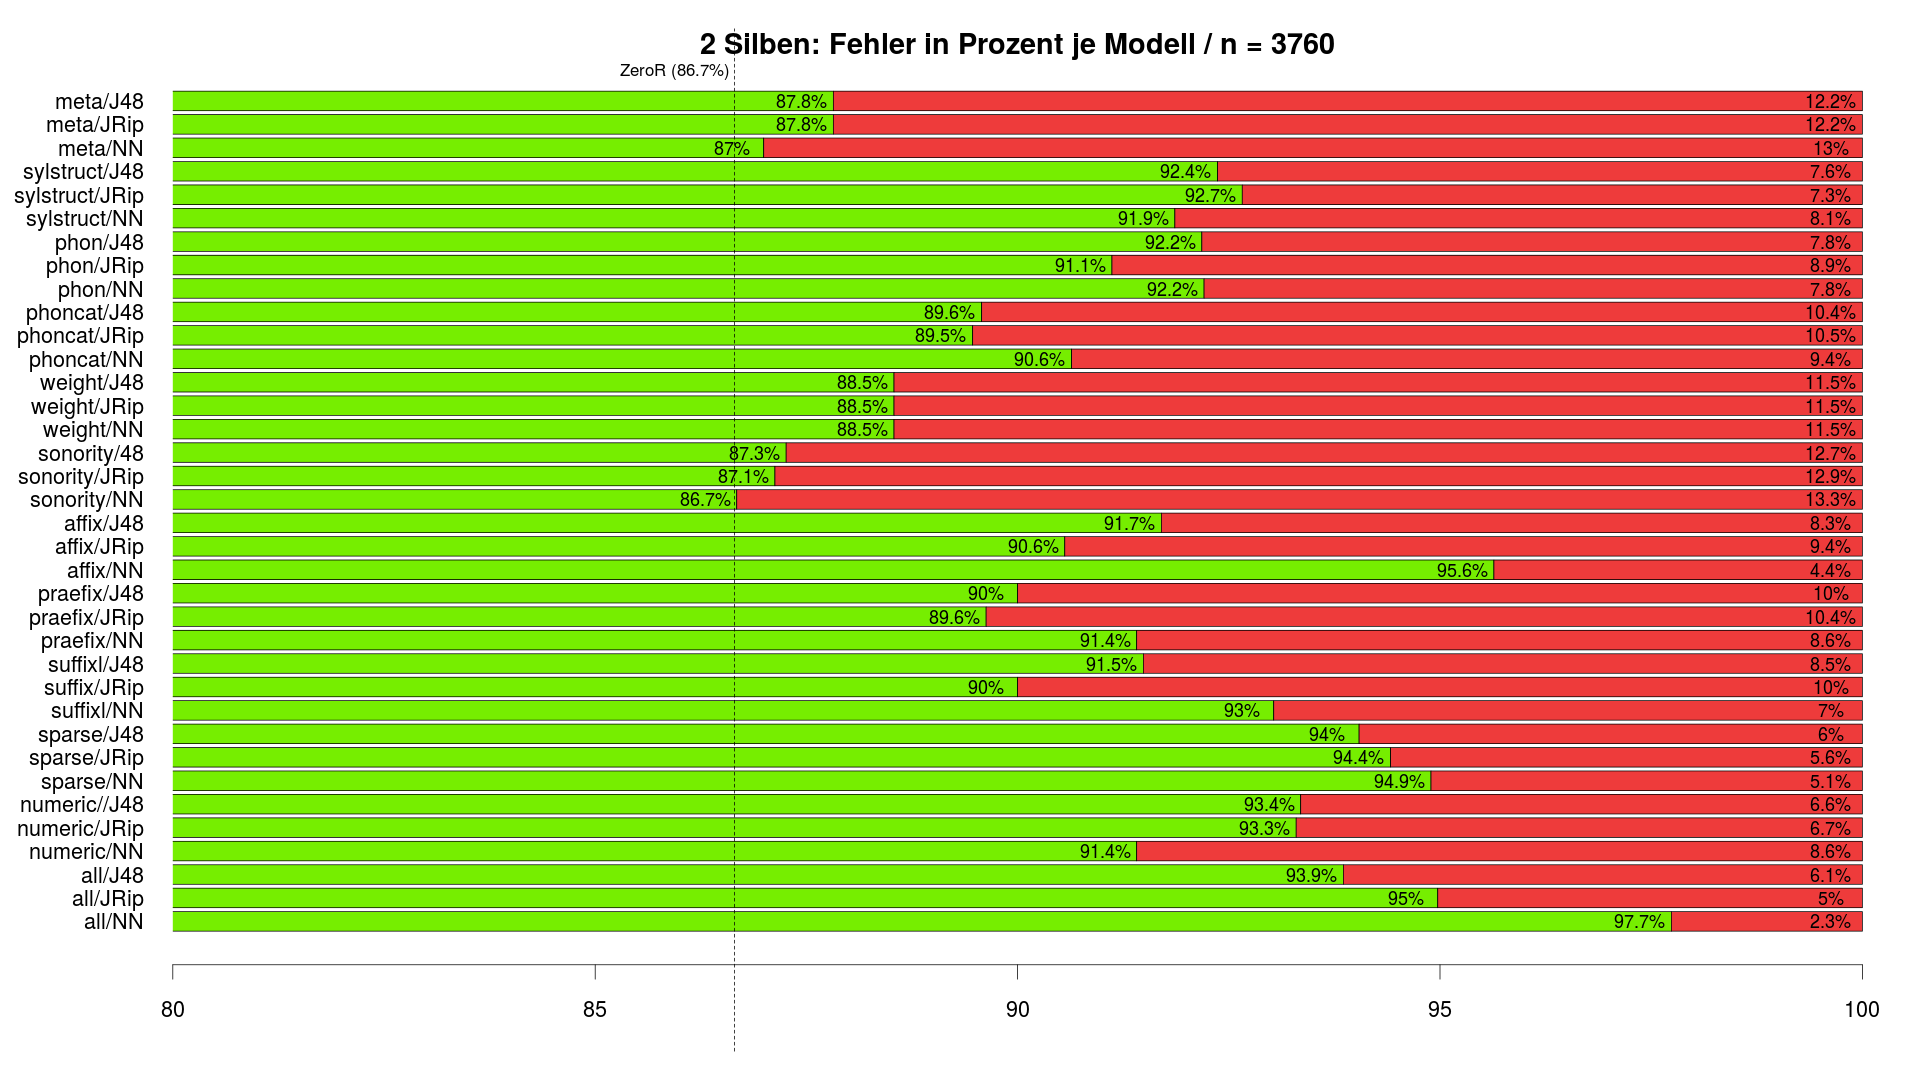
\includegraphics[width=12cm]{figures/basicstats/2syl-basicstats.png}}\end{center}
\begin{center}{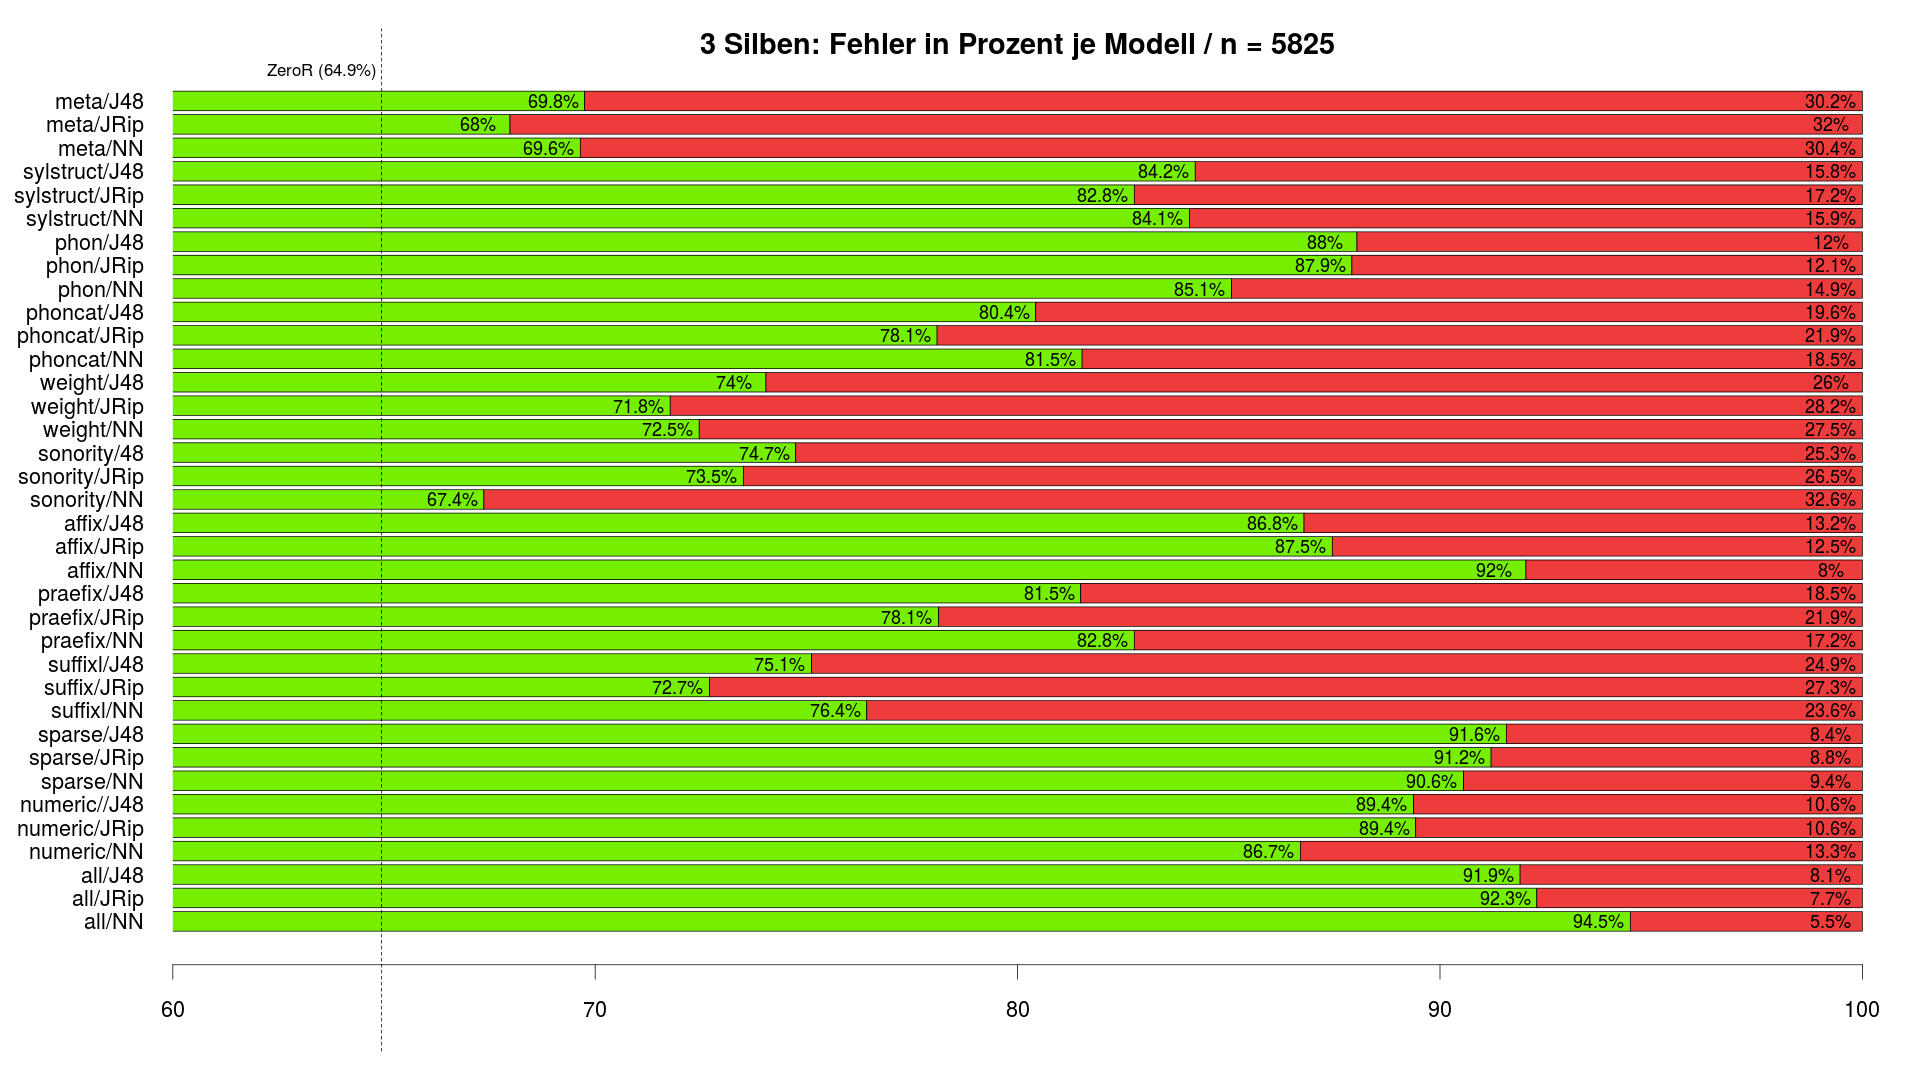
\includegraphics[width=12cm]{figures/basicstats/3syl-basicstats.png}}\end{center}
\begin{center}{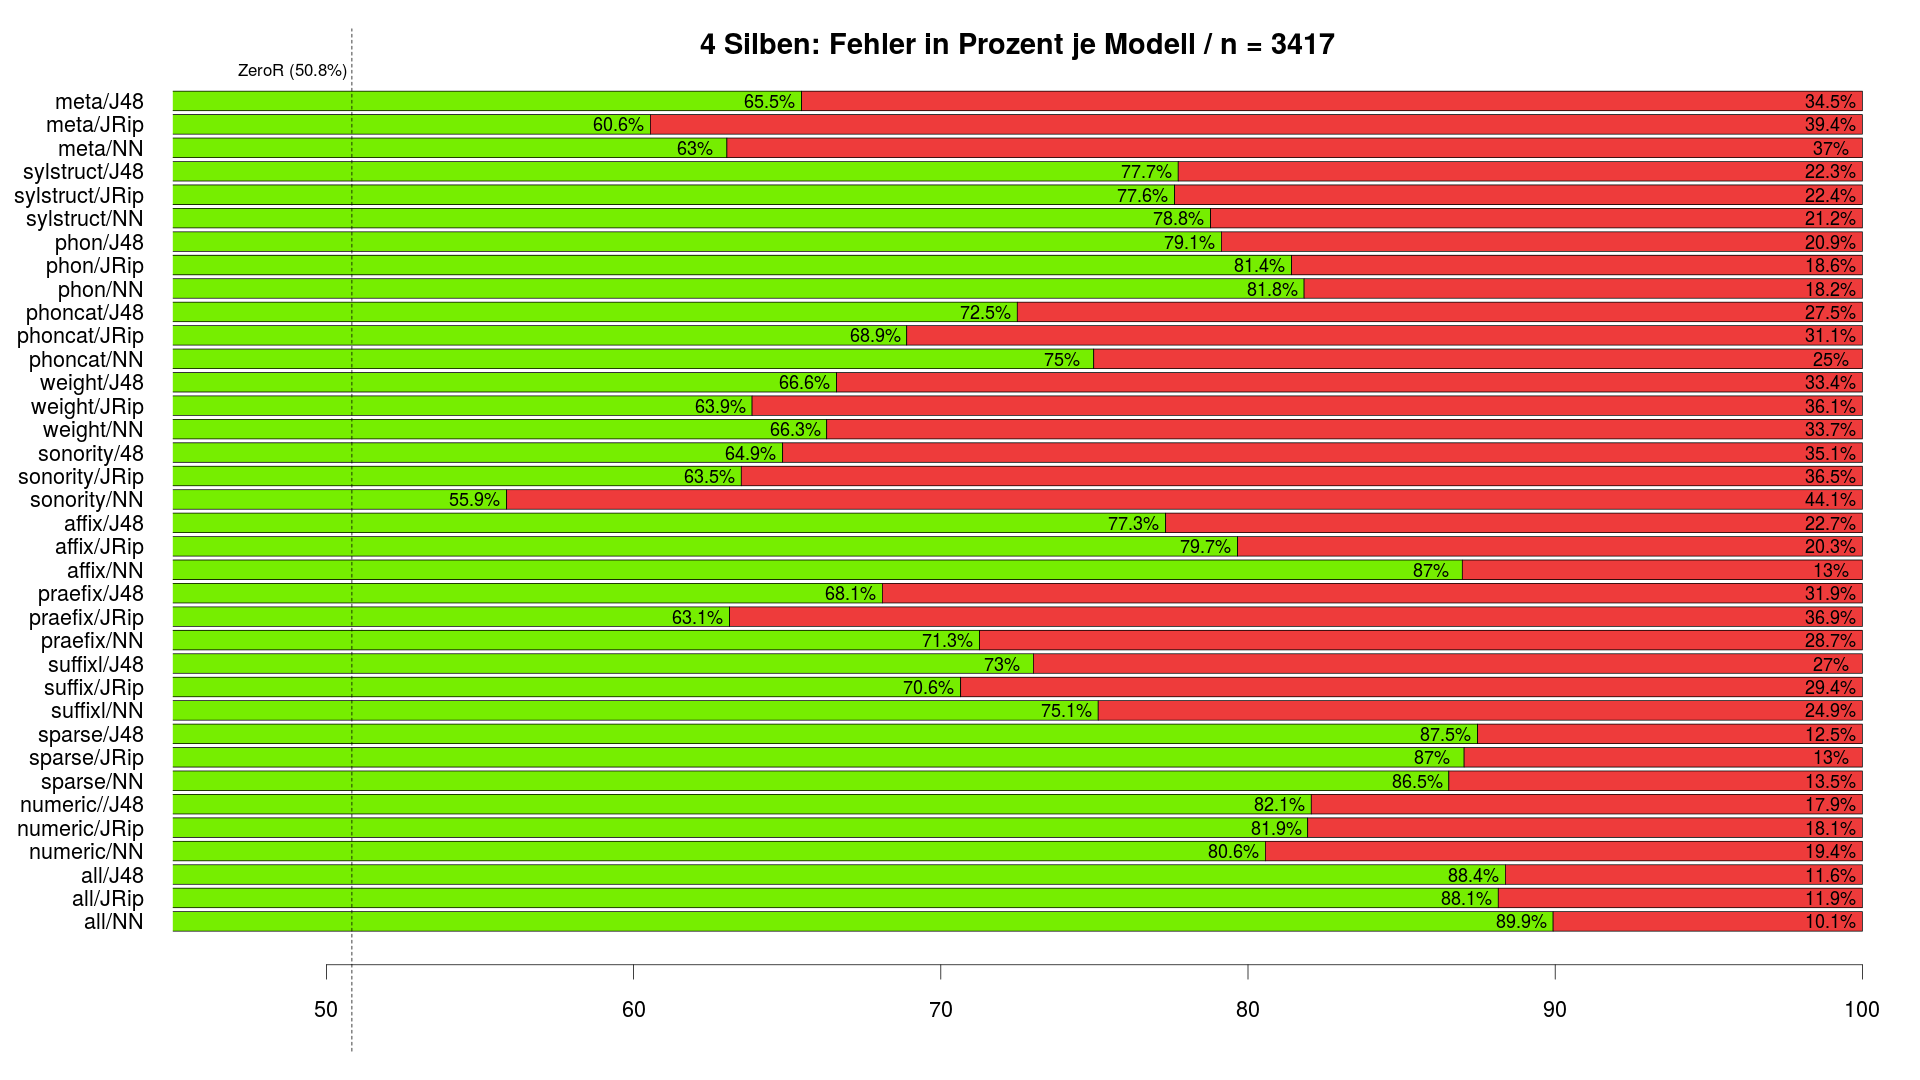
\includegraphics[width=12cm]{figures/basicstats/4syl-basicstats.png}}\end{center}
\begin{center}{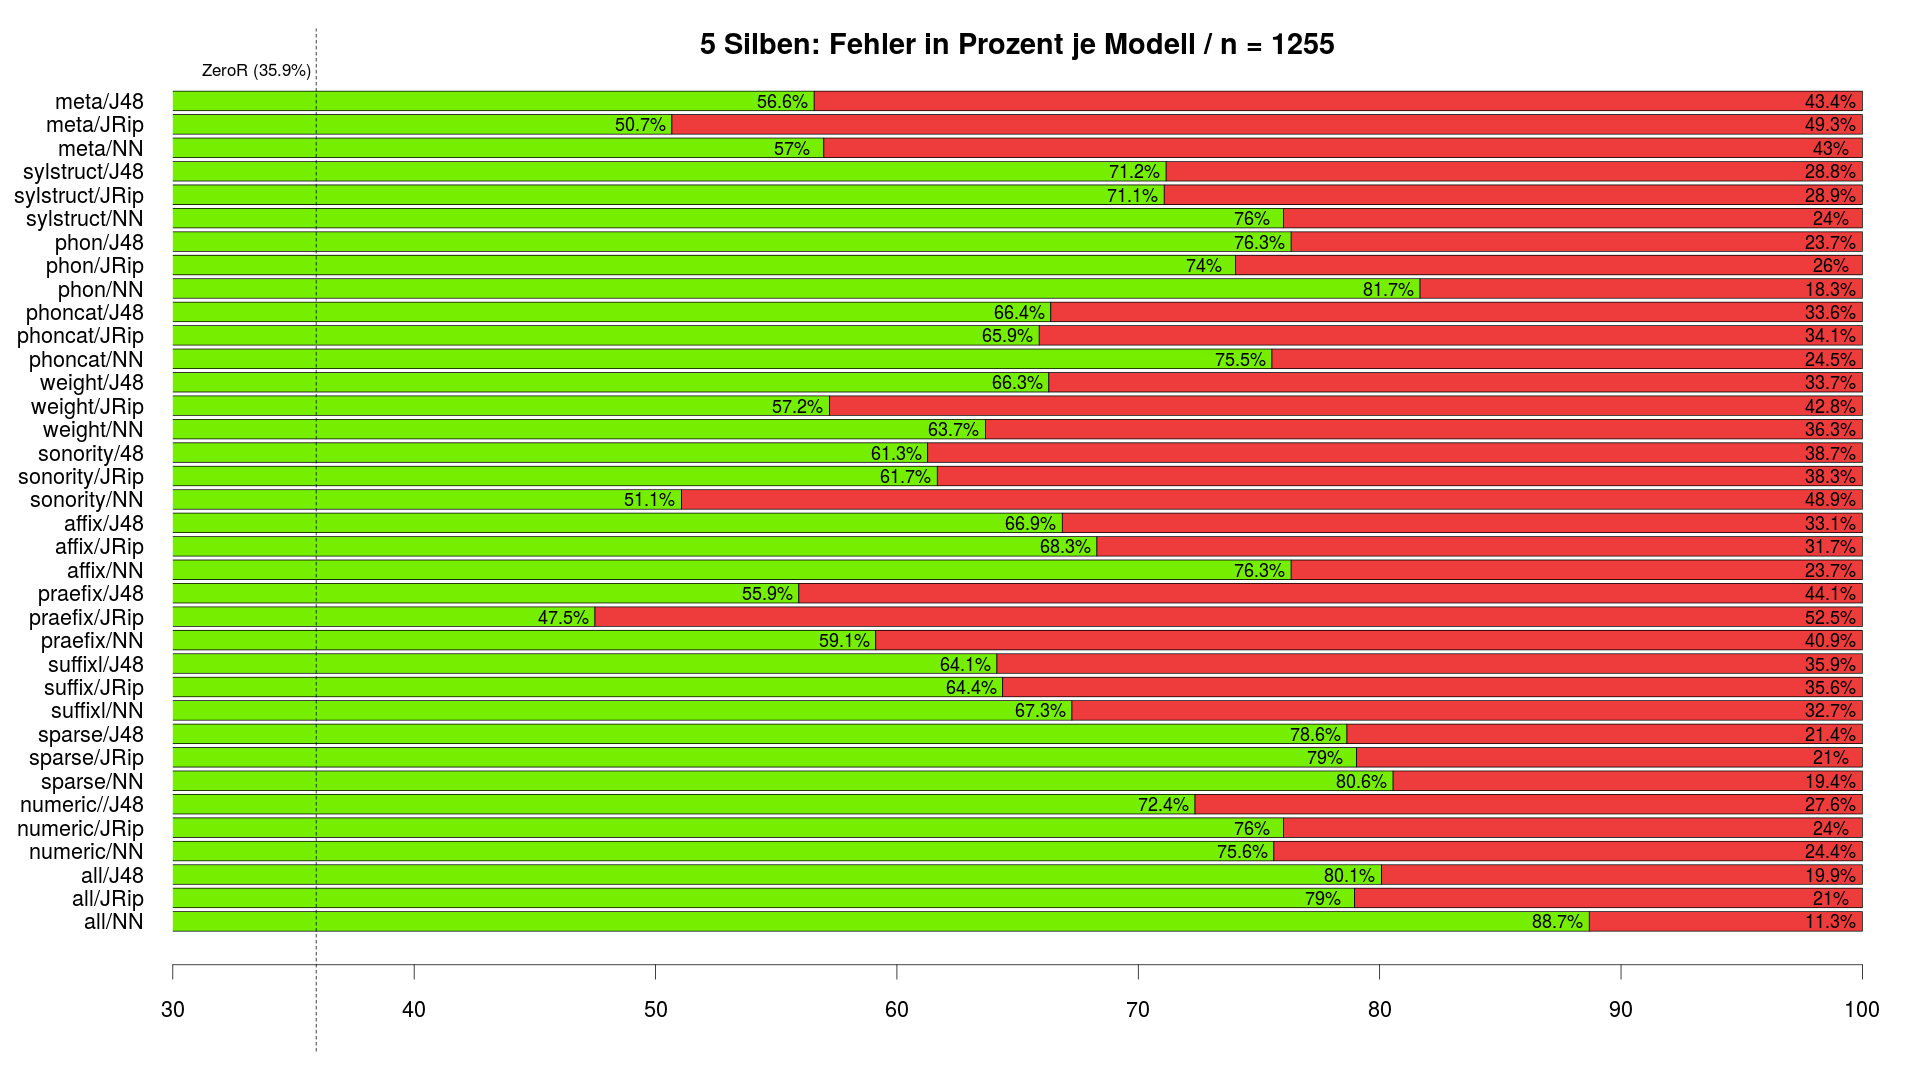
\includegraphics[width=12cm]{figures/basicstats/5syl-basicstats.png}}\end{center}
\begin{center}{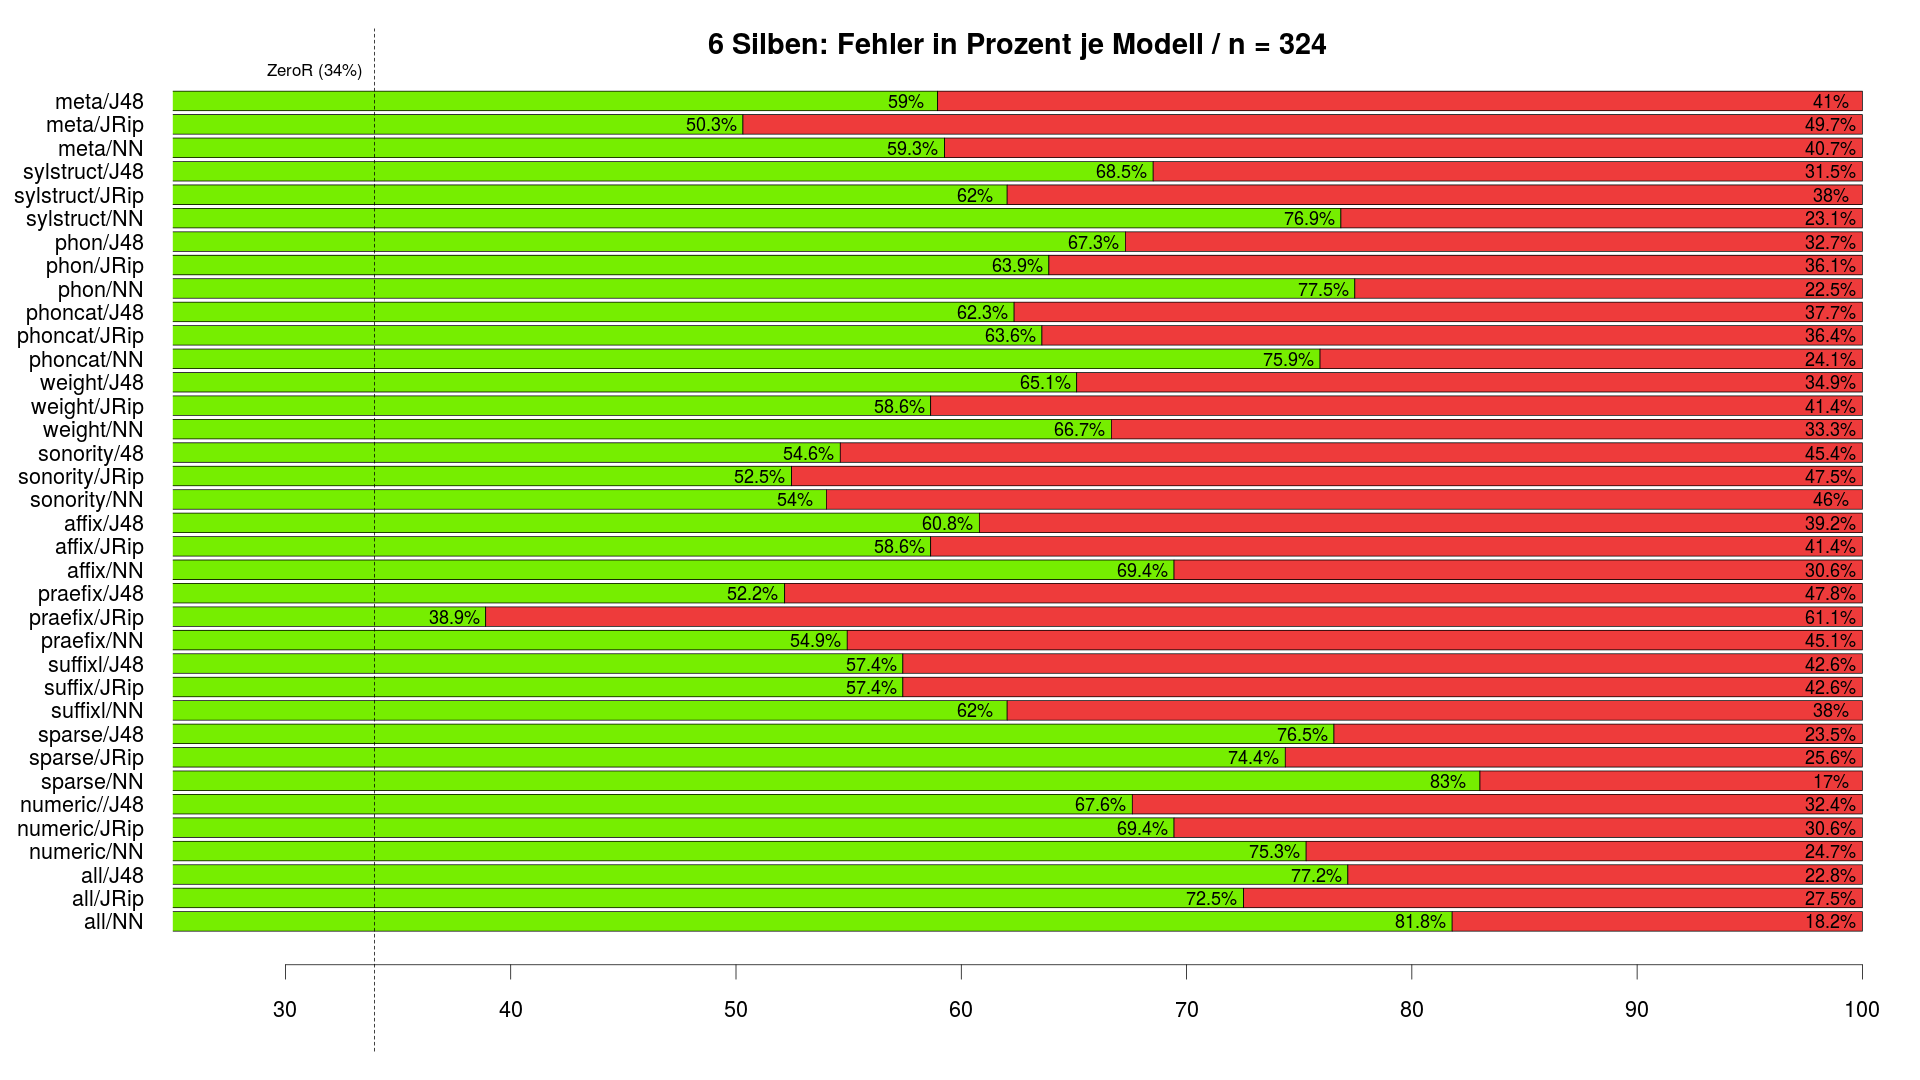
\includegraphics[width=12cm]{figures/basicstats/6syl-basicstats.png}}\end{center}
\begin{center}{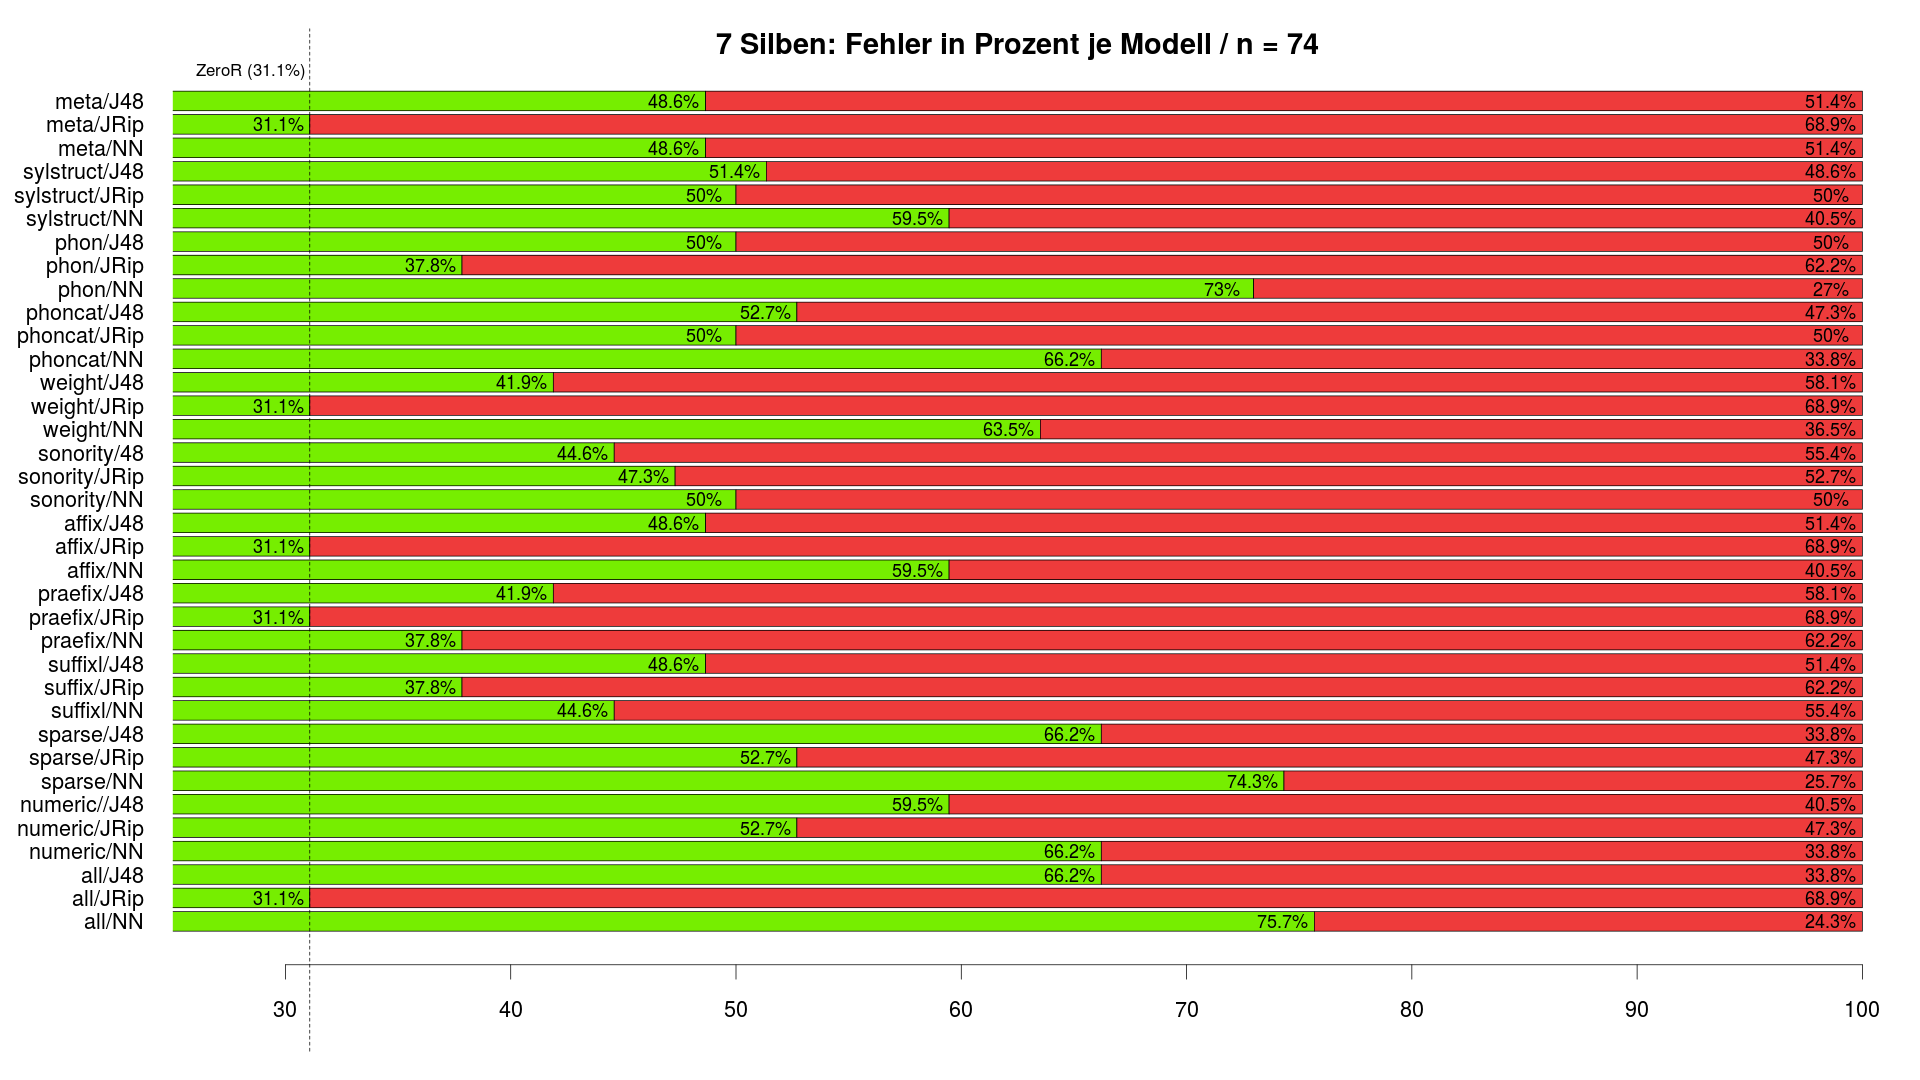
\includegraphics[width=12cm]{figures/basicstats/7syl-basicstats.png}}\end{center}
\newpage

%\section{Einfluss der Features}
\begin{figure}[!p]
    \begin{floatrow}
        \ffigbox{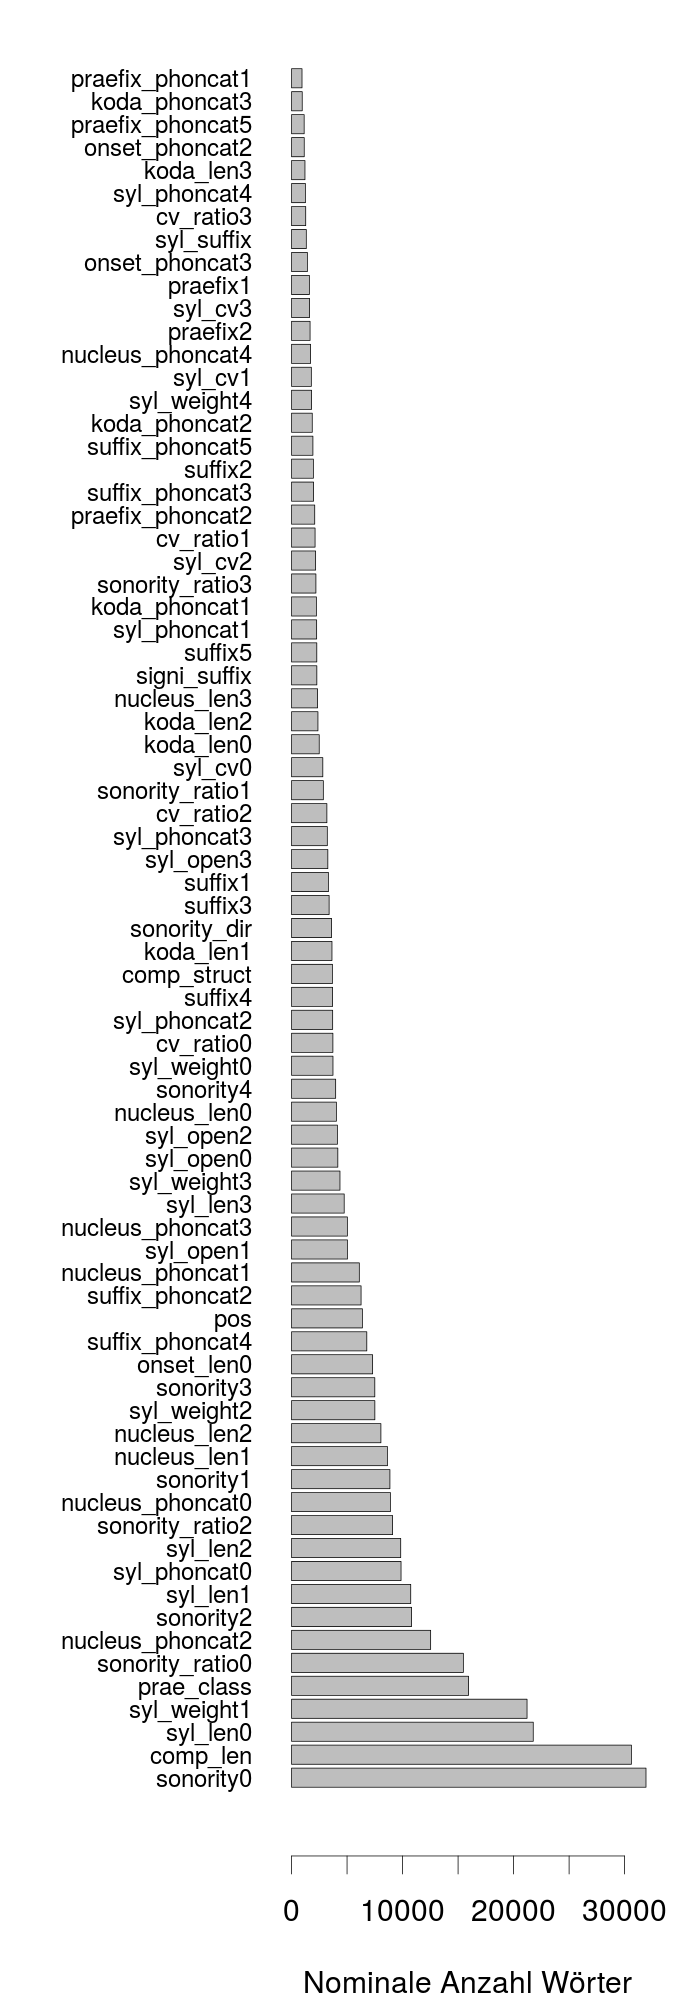
\includegraphics[scale = 0.27]{figures/features/jrip_feature_influence.png}} {
            \caption{75 häufigste Features}
            \label{figure:jrip_feature_influence}
        }
        \ffigbox{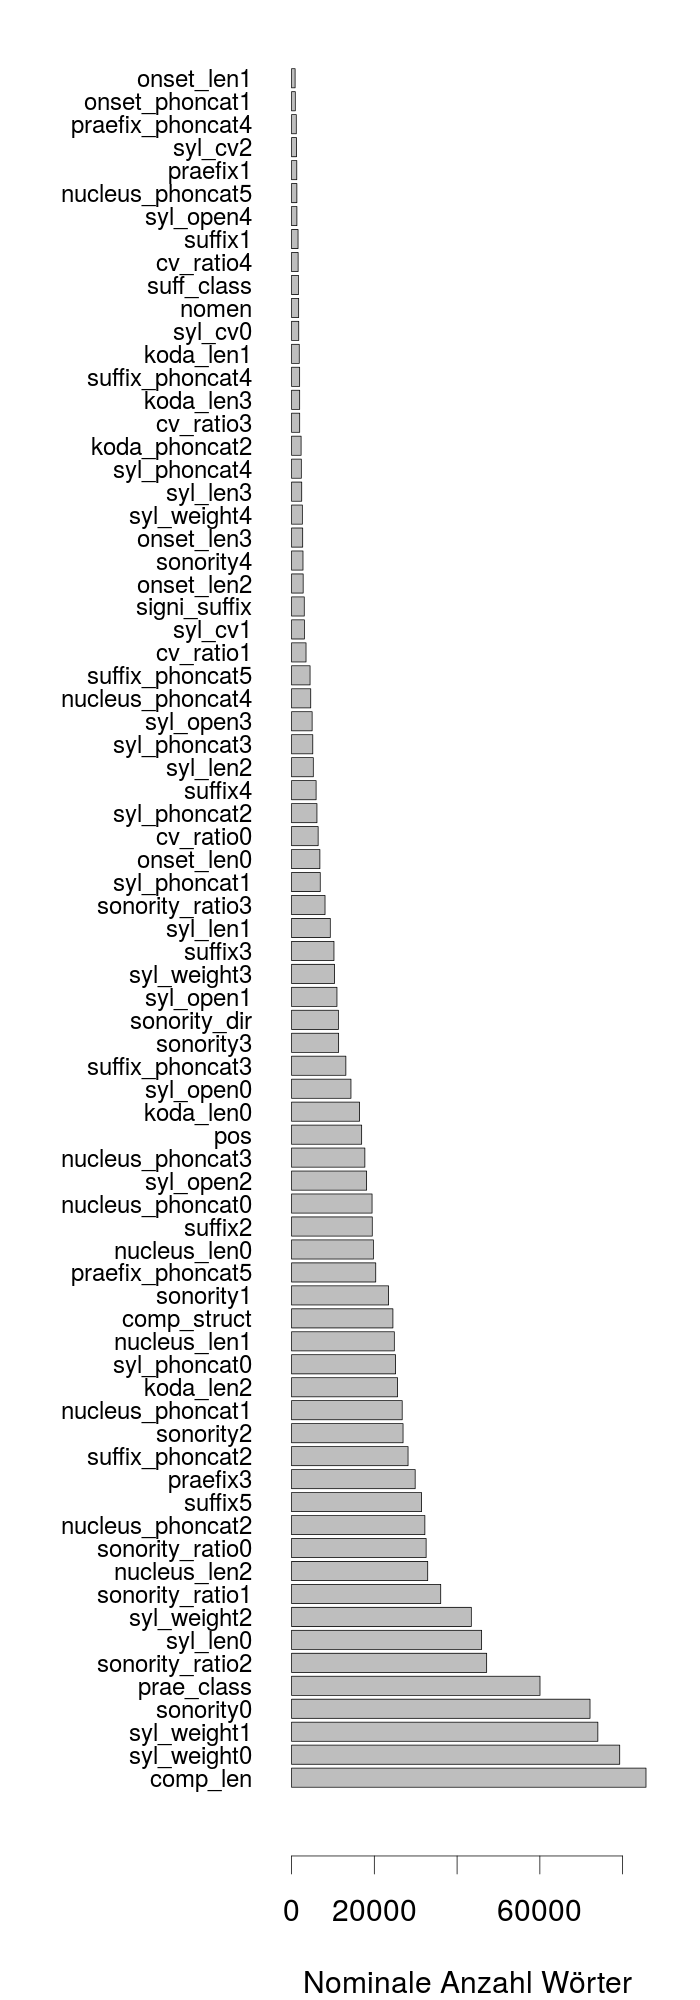
\includegraphics[scale = 0.27]{figures/features/j48_feature_influence.png}} {
            \caption{75 häufigste Features}
            \label{figure:j48_feature_influence}
        }
    \end{floatrow}
\end{figure}

%\section{Beispielregeln von JRip}
\begin{table}
\centering
\tiny
\caption{Die 50 einflussreichsten JRip-Regeln.}
\label{table:jrip_rules_examples}
\begin{tabular}{|p{8cm}l|ll|ll|}\hline
{\bf Regel} & {\bf Klasse} & {\bf TP} & {\bf FP} & {\bf Silben} & {\bf Featureset} \\\hline\hline
(prae\_class = noacc)                                                                                                                                                                                        & paenultima & 1562 & 1   & 3 & praefix   \\\hline
(prae\_class = noacc)                                                                                                                                                                                        & paenultima & 1561 & 1   & 3 & affix     \\\hline
(prae\_class = noacc)                                                                                                                                                                                        & paenultima & 1560 & 1   & 3 & all       \\\hline
(prae\_class = noacc)                                                                                                                                                                                        & paenultima & 1559 & 1   & 3 & sparse    \\\hline
(nucleus\_phoncat0 = K) and (syl\_phoncat0 = CK) and (nucleus\_phoncat2 = K)                                                                                                                                 & paenultima & 1137 & 271 & 3 & phoncat   \\\hline
(nucleus\_phoncat0 = K) and (syl\_phoncat2 = CKC) and (syl\_phoncat0 = CKC)                                                                                                                                  & paenultima & 1069 & 388 & 3 & phoncat   \\\hline
(syl\_cv0 = CVC) and (nucleus\_len1 \textgreater= 2) and (syl\_len0 \textless= 3)                                                                                                                            & paenultima & 896  & 175 & 3 & sylstruct \\\hline
(nucleus\_phoncat0 = K) and (syl\_weight1 = light) and (sonority0 \textless= 11) and (sonority0 \textgreater= 10) and (syl\_phoncat0 = CKC) and (sonority0 \textgreater= 11)                                 & paenultima & 877  & 95  & 3 & phon      \\\hline
(sonority0 \textless= 11) and (sonority\_ratio0 \textless= 3) and (sonority\_ratio0 \textgreater= 3) and (sonority0 \textgreater= 11) and (sonority1 \textgreater= 11) and (sonority2 \textgreater= 10)      & paenultima & 738  & 217 & 3 & sonority  \\\hline
(comp\_len \textless= 1) and (cv\_ratio0 \textgreater= 2) and (syl\_len0 \textless= 3) and (sonority\_ratio0 \textless= 3) and (nucleus\_len1 \textgreater= 2)                                               & paenultima & 729  & 45  & 3 & numeric   \\\hline
(syl\_weight0 = schwa)                                                                                                                                                                                       & paenultima & 721  & 0   & 3 & weight    \\\hline
(nucleus\_phoncat0 = K) and (syl\_open0 = o)                                                                                                                                                                 & paenultima & 716  & 0   & 3 & phon      \\\hline
(nucleus\_len0 \textless= 1) and (syl\_len0 \textless= 3) and (syl\_cv0 = CV)                                                                                                                                & paenultima & 713  & 0   & 3 & sylstruct \\\hline
(comp\_len \textless= 1) and (sonority\_ratio0 \textless= 3) and (koda\_len0 \textless= 0) and (nucleus\_len0 \textless= 1)                                                                                  & paenultima & 664  & 0   & 3 & numeric   \\\hline
(comp\_len \textless= 1) and (nucleus\_len2 \textgreater= 2) and (cv\_ratio1 \textless= 0)                                                                                                                   & paenultima & 647  & 83  & 4 & numeric   \\\hline
(syl\_len0 \textless= 3) and (nucleus\_len0 \textless= 1) and (syl\_cv2 = CVC) and (syl\_len0 \textgreater= 3) and (koda\_len1 \textgreater= 1)                                                              & paenultima & 637  & 174 & 3 & sylstruct \\\hline
(nucleus\_phoncat3 = L) and (nucleus\_phoncat2 = L)                                                                                                                                                          & paenultima & 610  & 167 & 5 & phoncat   \\\hline
(nucleus\_len2 \textgreater= 2) and (comp\_len \textless= 1) and (signi\_suffix = ø) and (suffix\_phoncat2 = LC) and (syl\_weight1 = light)                                                                  & ultima     & 595  & 56  & 3 & all       \\\hline
(nucleus\_phoncat2 = L) and (nucleus\_phoncat1 = L) and (syl\_phoncat3 = CKC)                                                                                                                                & paenultima & 558  & 71  & 4 & phoncat   \\\hline
(sonority0 \textless= 11) and (sonority\_ratio0 \textless= 3) and (sonority\_ratio0 \textgreater= 3) and (sonority\_ratio2 \textgreater= 4) and (sonority\_dir \textless= 1) and (sonority1 \textgreater= 8) & paenultima & 544  & 204 & 3 & sonority  \\\hline
(nucleus\_len2 \textgreater= 2) and (comp\_len \textless= 1) and (syl\_len1 \textless= 2) and (onset\_len0 \textgreater= 1) and (syl\_len2 \textgreater= 3)                                                  & ultima     & 516  & 44  & 3 & sparse    \\\hline
(nucleus\_len2 \textgreater= 2) and (comp\_len \textless= 1) and (syl\_len1 \textless= 2) and (onset\_len0 \textgreater= 1) and (syl\_len2 \textgreater= 3)                                                  & ultima     & 516  & 44  & 3 & numeric   \\\hline
(nucleus\_phoncat3 = L) and (comp\_len \textless= 1) and (signi\_suffix = ø) and (syl\_len3 \textgreater= 3)                                                                                                 & ultima     & 498  & 56  & 4 & all       \\\hline
(syl\_weight1 = light) and (nucleus\_phoncat2 = L) and (syl\_phoncat4 = CKC)                                                                                                                                 & paenultima & 490  & 86  & 5 & phon     \\\hline
(suffix\_phoncat4 = LCKC) and (suffix4 = eren)                                                                                                                                                                                                              & paenultima     & 477 & 50  & 4 & suffix    \\\hline
(nucleus\_phoncat3 = L) and (comp\_len \textless= 1) and (syl\_len2 \textless= 2) and (koda\_phoncat3 = C)                                                                                                                                                  & ultima         & 477 & 38  & 4 & sparse    \\\hline
(nucleus\_phoncat1 = L) and (nucleus\_phoncat2 = L) and (onset\_phoncat3 = C) and (syl\_open1 = o)                                                                                                                                                          & paenultima     & 463 & 77  & 4 & phon      \\\hline
(syl\_weight1 = light) and (nucleus\_phoncat2 = L) and (sonority0 \textless= 10) and (sonority3 \textgreater= 13)                                                                                                                                           & paenultima     & 454 & 44  & 4 & phon      \\\hline
(comp\_len \textless= 1) and (sonority0 \textless= 10) and (sonority0 \textgreater= 10) and (onset\_len0 \textless= 0) and (nucleus\_len0 \textless= 1)                                                                                                     & paenultima     & 450 & 23  & 3 & numeric   \\\hline
(sonority\_ratio0 \textless= 4) and (sonority2 \textgreater= 10) and (sonority\_ratio2 \textless= 4) and (sonority0 \textless= 11)                                                                                                                          & sekunda        & 447 & 197 & 5 & sonority  \\\hline
(comp\_len \textless= 1) and (cv\_ratio0 \textgreater= 2) and (sonority0 \textless= 11) and (sonority0 \textgreater= 11) and (koda\_len1 \textgreater= 1) and (nucleus\_len2 \textless= 1) and (syl\_len0 \textless= 3) and (sonority\_ratio0 \textless= 3) & paenultima     & 435 & 12  & 3 & numeric   \\\hline
(nucleus\_len2 \textgreater= 2) and (syl\_cv1 = CVV) and (koda\_len2 \textgreater= 1)                                                                                                                                                                       & ultima         & 428 & 80  & 3 & sylstruct \\\hline
(suffix\_phoncat4 = LCKC) and (suffix5 = ieren) and (prae\_class = ø)                                                                                                                                                                                       & paenultima     & 426 & 4   & 4 & affix     \\\hline
(sonority\_dir \textgreater= 1) and (sonority\_ratio2 \textgreater= 4) and (sonority3 \textgreater= 13) and (sonority3 \textless= 13)                                                                                                                       & paenultima     & 425 & 106 & 4 & sonority  \\\hline
(syl\_weight3 = light) and (syl\_open2 = o) and (syl\_weight2 = light) and (syl\_weight1 = light) and (syl\_open0 = o)                                                                                                                                      & ultima         & 416 & 207 & 4 & weight    \\\hline
(syl\_len0 \textless= 2) and (nucleus\_len1 \textgreater= 2) and (onset\_len0 \textgreater= 1) and (onset\_len2 \textgreater= 1)                                                                                                                            & paenultima     & 412 & 113 & 3 & numeric   \\\hline
(comp\_len \textless= 1) and (sonority0 \textless= 10) and (nucleus\_phoncat2 = L) and (syl\_weight1 = light) and (sonority1 \textless= 10) and (onset\_phoncat3 = C)                                                                                       & paenultima     & 398 & 37  & 4 & all       \\\hline
(prae\_class = noacc)                                                                                                                                                                                                                                       & antepaenultima & 392 & 2   & 4 & sparse    \\\hline
(prae\_class = noacc)                                                                                                                                                                                                                                       & antepaenultima & 392 & 2   & 4 & praefix   \\\hline
(prae\_class = noacc)                                                                                                                                                                                                                                       & antepaenultima & 392 & 2   & 4 & all       \\\hline
(prae\_class = noacc)                                                                                                                                                                                                                                       & antepaenultima & 390 & 2   & 4 & affix     \\\hline
(syl\_suffix = ø) and (comp\_len \textless= 1) and (syl\_weight2 = heavy) and (syl\_weight1 = light)                                                                                                                                                        & ultima         & 382 & 74  & 3 & all       \\\hline
(sonority0 \textless= 11) and (syl\_weight1 = light) and (syl\_open0 = o) and (syl\_phoncat0 = CL) and (onset\_phoncat2 = C) and (nucleus\_phoncat2 = K)                                                                                                    & paenultima     & 378 & 103 & 3 & phon      \\\hline
(sonority0 \textless= 10) and (syl\_weight1 = light) and (sonority0 \textgreater= 10) and (nucleus\_phoncat0 = K) and (sonority\_ratio0 \textgreater= 5)                                                                                                    & paenultima     & 370 & 31  & 3 & phon      \\\hline
(syl\_len0 \textless= 2) and (nucleus\_len2 \textgreater= 2) and (nucleus\_len1 \textgreater= 2) and (syl\_cv3 = CVC) and (syl\_len1 \textless= 3)                                                                                                          & paenultima     & 364 & 39  & 4 & sylstruct \\\hline
(nucleus\_phoncat2 = L) and (syl\_phoncat1 = CL) and (koda\_phoncat2 = C)                                                                                                                                                                                   & ultima         & 359 & 60  & 3 & phoncat   \\\hline
(comp\_len \textless= 1) and (sonority0 \textless= 10) and (syl\_weight1 = light) and (prae\_class = ø) and (syl\_weight3 = schwa)                                                                                                                          & paenultima     & 359 & 50  & 4 & sparse    \\\hline
\end{tabular}
\end{table}
\begin{landscape}
\begin{table}[p]
\centering
\tiny
\caption{Drei Beispiele für die Wörter \textit{knifflig, ruecklings} und \textit{trennen} aus dem Trainingsset der Zweisilber.}
\label{table:data_example}
\begin{tabular}{|p{2cm}|p{2cm}|p{2cm}|p{2cm}|p{2cm}|p{1.5cm}|p{1.5cm}|p{1.5cm}|p{1.8cm}|p{1.8cm}|}
\hline
{\bf syl\_suffix}       & {\bf signi\_suffix}     & {\bf suffix1}           & {\bf suffix2}           & {\bf suffix3}           & {\bf suffix4}       & {\bf suffix5}       & {\bf suffix\_phoncat1} & {\bf suffix\_phoncat2} & {\bf suffix\_phoncat3} \\\hline
ø                       & ø                       & g                       & ig                      & lig                     & ø                   & ø                   & C                      & KC                     & CKC                    \\
ø                       & ø                       & s                       & ø                       & ø                       & ø                   & ø                   & C                      & CC                     & KCC                    \\
nen                     & ø                       & n                       & en                      & nen                     & ø                   & ø                   & C                      & KC                     & CKC                    \\\hline
\hline
{\bf suffix\_phoncat4}  & {\bf suffix\_phoncat5}  & {\bf suff\_class}       & {\bf syl\_praefix}      & {\bf signi\_praefix}    & {\bf praefix1}      & {\bf praefix2}      & {\bf praefix3}         & {\bf praefix4}         & {\bf praefix5}         \\
CCKC                    & KCCKC                   & ø                       & ø                       & ø                       & k                   & kn                  & ø                      & ø                      & ø                      \\
CKCC                    & CCKCC                   & ø                       & ø                       & ø                       & r                   & ru                  & ø                      & ø                      & ø                      \\
KCKC                    & CKCKC                   & ø                       & ø                       & ø                       & t                   & tr                  & ø                      & ø                      & ø                      \\\hline
\hline
{\bf praefix\_phoncat1} & {\bf praefix\_phoncat2} & {\bf praefix\_phoncat3} & {\bf praefix\_phoncat4} & {\bf praefix\_phoncat5} & {\bf prae\_class}   & {\bf sonority0}     & {\bf sonority1}        & {\bf sonority\_ratio0} & {\bf sonority\_ratio1} \\
C                       & CC                      & CCK                     & CCKC                    & CCKCC                   & ø                   & 13                  & 13                     & 3                      & 4                      \\
C                       & CK                      & CKC                     & CKCC                    & CKCCK                   & ø                   & 13                  & 16                     & 4                      & 4                      \\
C                       & CC                      & CCK                     & CCKC                    & CCKCK                   & ø                   & 11                  & 12                     & 3                      & 4                      \\\hline
\hline
{\bf sonority\_dir}     & {\bf syl\_weight0}      & {\bf syl\_weight1}      & {\bf syl\_open0}        & {\bf syl\_open1}        & {\bf syl\_phoncat0} & {\bf syl\_phoncat1} & {\bf onset\_phoncat0}  & {\bf onset\_phoncat1}  & {\bf koda\_phoncat0}   \\
0                       & light                   & light                   & c                       & c                       & CCKC                & CKC                 & CC                     & C                      & C                      \\
2                       & light                   & heavy                   & c                       & c                       & CKC                 & CKCC                & C                      & C                      & C                      \\
1                       & light                   & schwa                   & c                       & c                       & CCK                 & CKC                 & CC                     & C                      & ø                      \\\hline
\hline
{\bf koda\_phoncat1}    & {\bf nucleus\_phoncat0} & {\bf nucleus\_phoncat1} & {\bf syl\_len0}         & {\bf syl\_len1}         & {\bf koda\_len0}    & {\bf koda\_len1}    & {\bf onset\_len0}      & {\bf onset\_len1}      & {\bf nucleus\_len0}    \\
C                       & K                       & K                       & 4                       & 4                       & 1                   & 1                   & 2                      & 1                      & 1                      \\
CC                      & K                       & K                       & 4                       & 5                       & 1                   & 2                   & 1                      & 1                      & 1                      \\
C                       & K                       & K                       & 4                       & 3                       & 1                   & 1                   & 2                      & 1                      & 1                      \\\hline
\hline
{\bf nucleus\_len1}     & {\bf syl\_cv0}          & {\bf syl\_cv1}          & {\bf cv\_ratio0}        & {\bf cv\_ratio1}        & {\bf pos}           & {\bf comp\_struct}  & {\bf nomen}            & {\bf comp\_len}        & {\bf stress\_class}    \\
1                       & CCVC                    & CVC                     & 3                       & 2                       & A                   & V                   & F                      & 1                      & paenultima             \\
1                       & CVC                     & CVCC                    & 2                       & 3                       & ADV                 & N                   & F                      & 1                      & paenultima             \\
1                       & CCVC                    & CVC                     & 3                       & 2                       & V                   & V                   & F                      & 1                      & paenultima            \\\hline
\end{tabular}
\end{table}
\end{landscape}

%%%%%%%%%%%%%%%%%%%%%

%\begin{landscape}
%\section{Vergleich der Modelle}

%\begin{center}{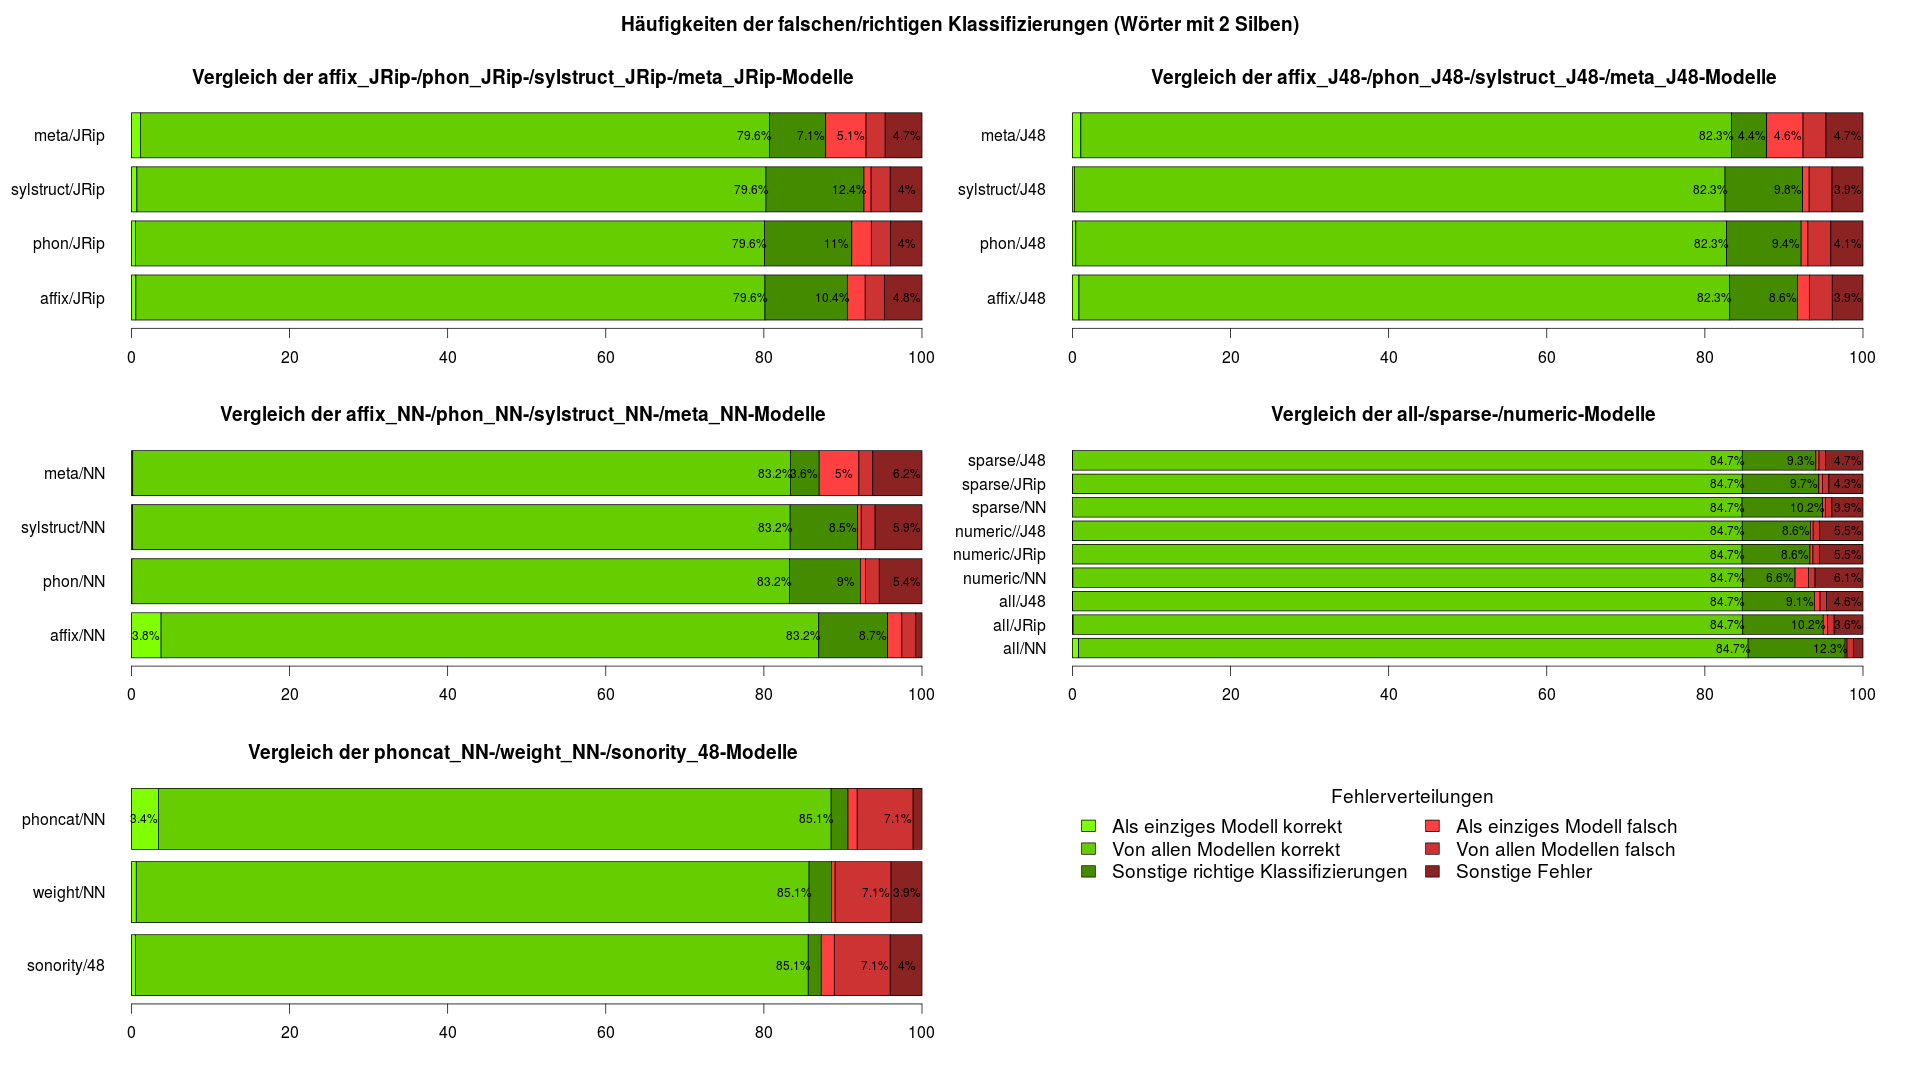
\includegraphics[width=22cm]{figures/compare/2syl.png}}\end{center}
%\begin{center}{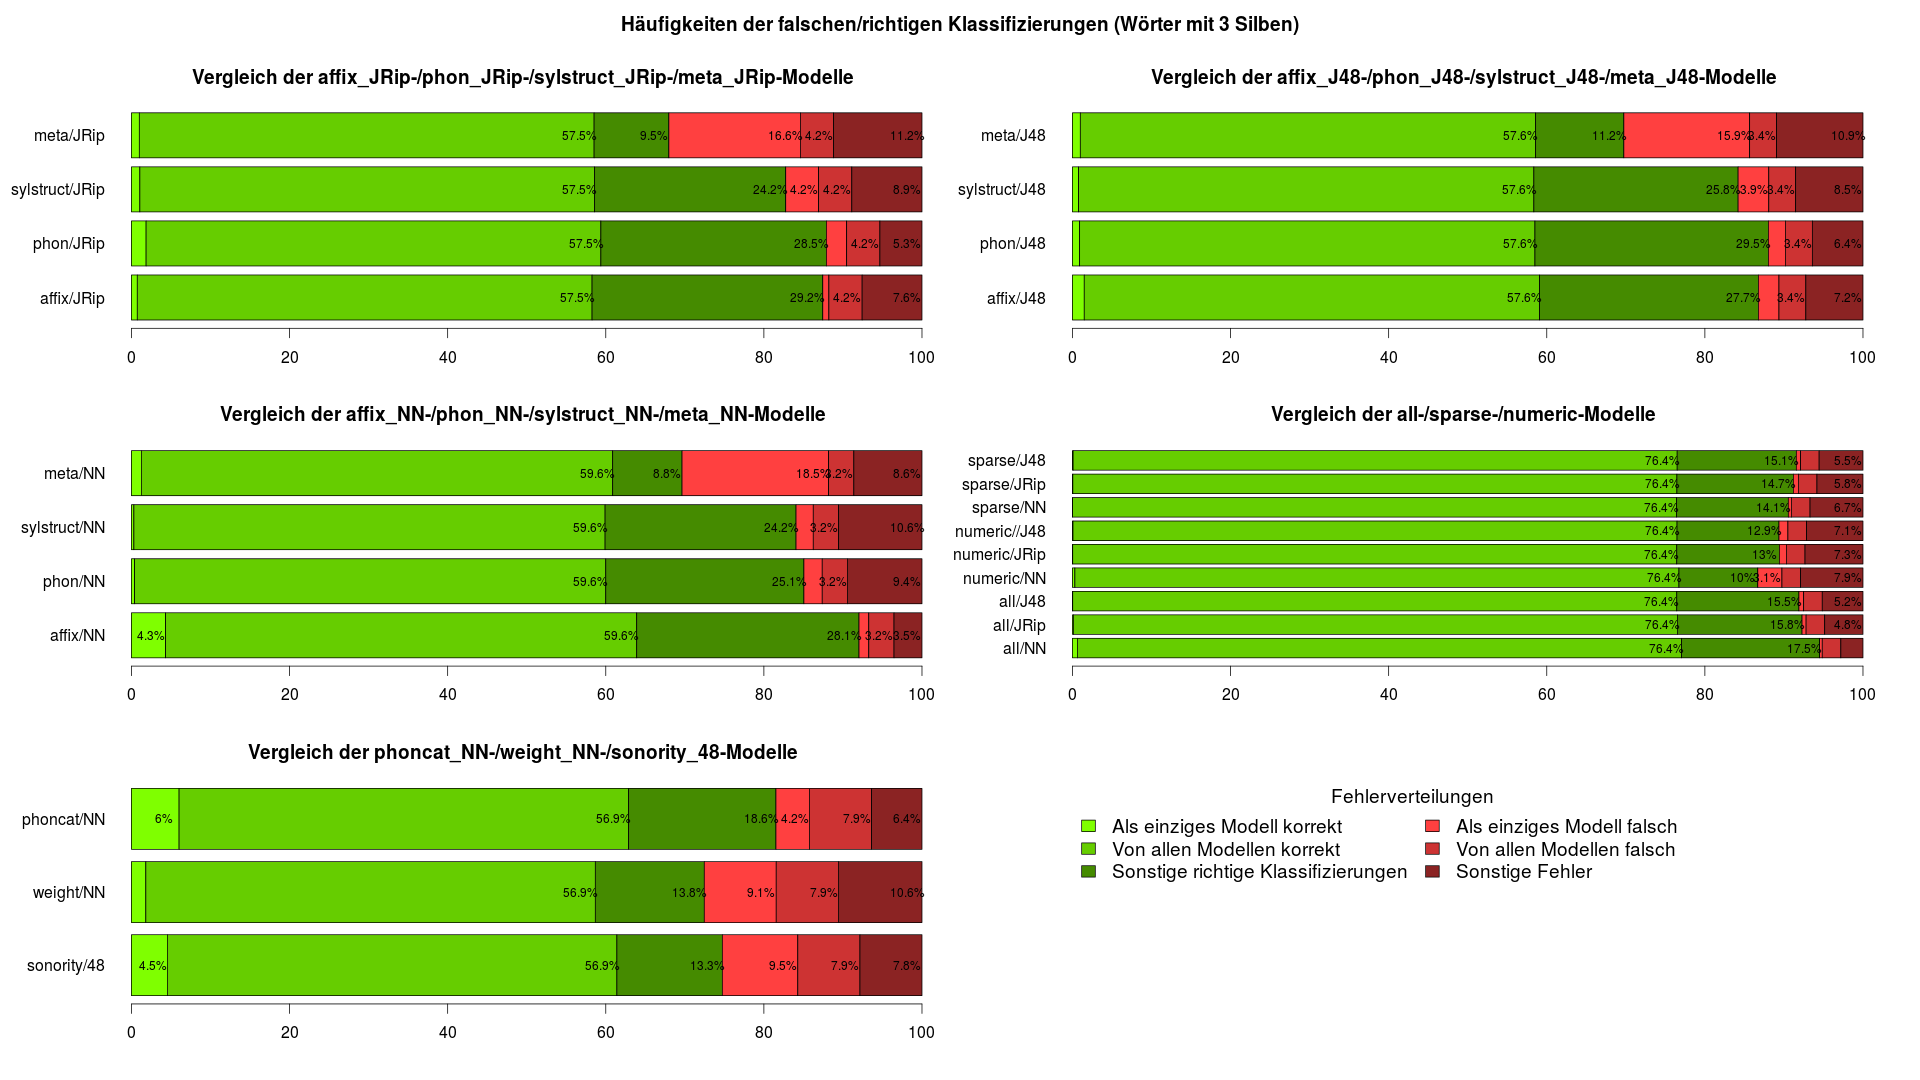
\includegraphics[width=22cm]{figures/compare/3syl.png}}\end{center}
%\begin{center}{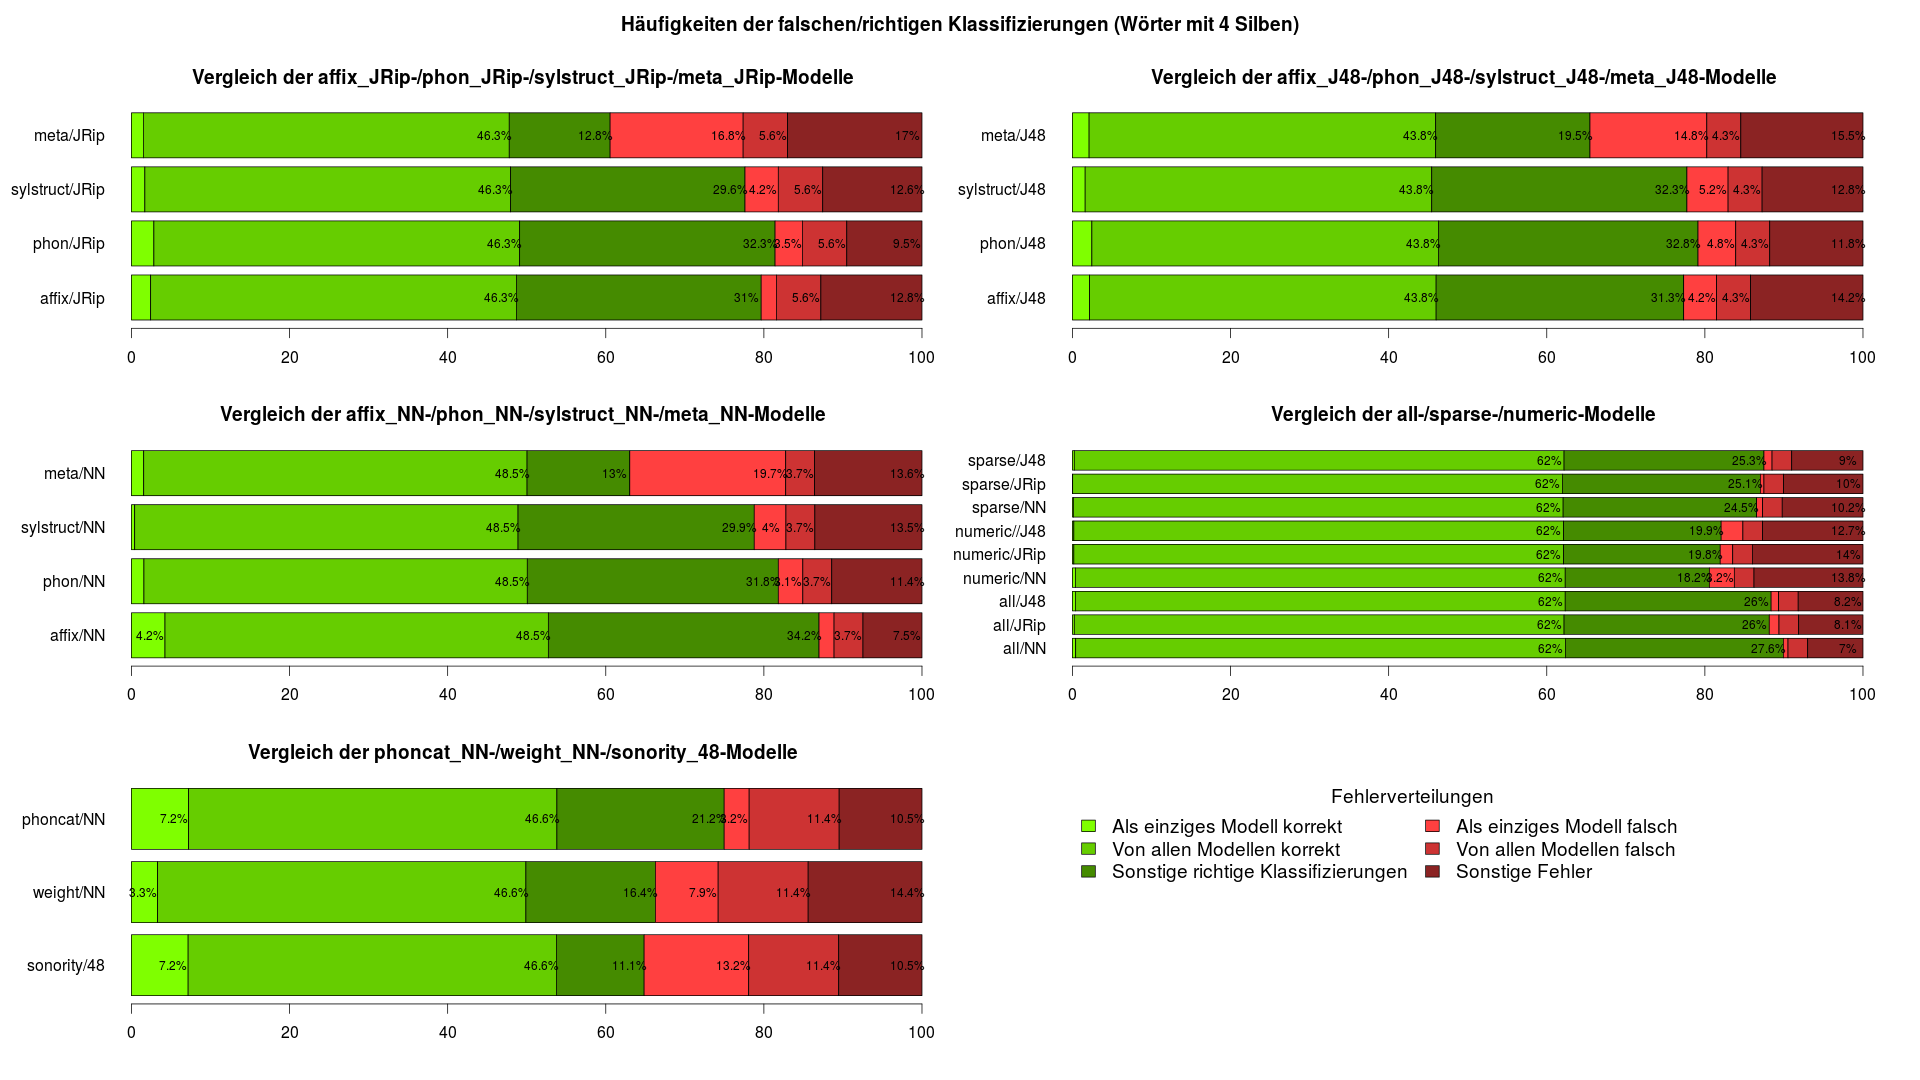
\includegraphics[width=22cm]{figures/compare/4syl.png}}\end{center}
%\begin{center}{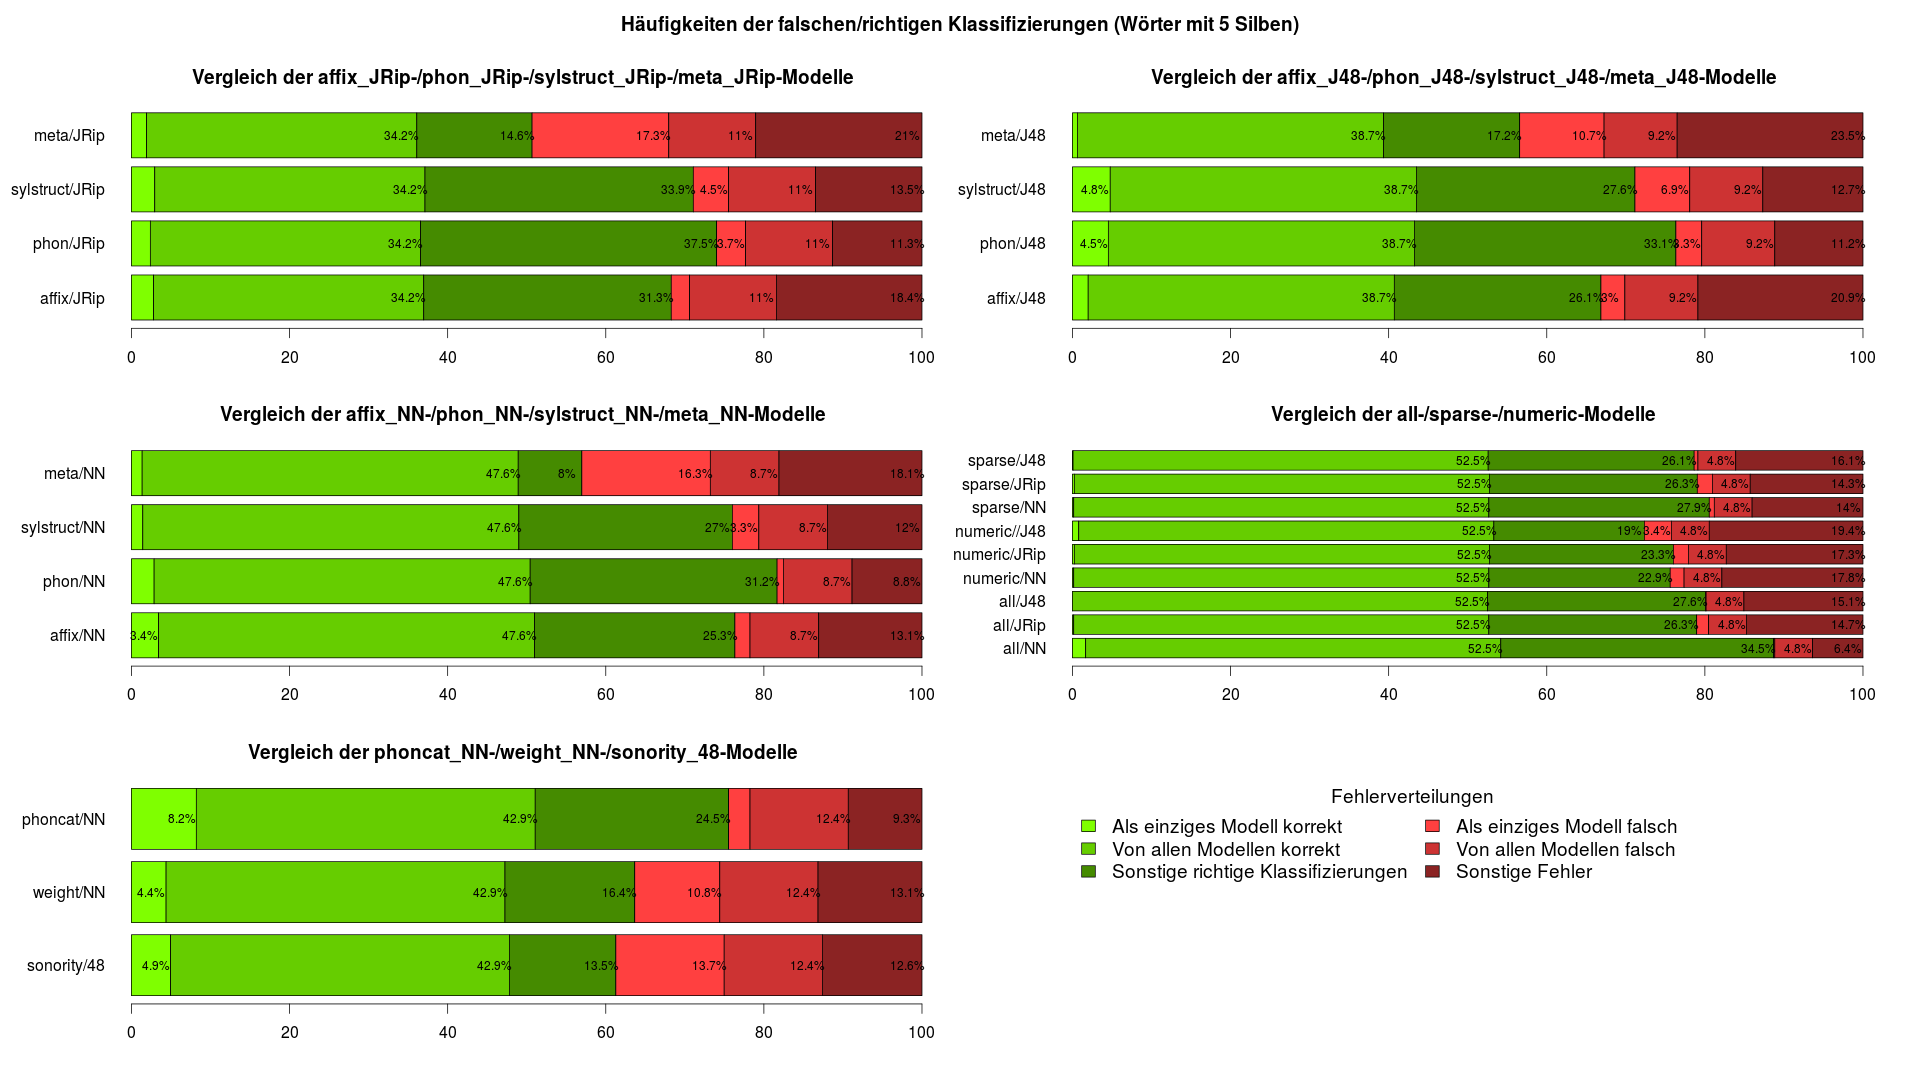
\includegraphics[width=22cm]{figures/compare/5syl.png}}\end{center}
%\begin{center}{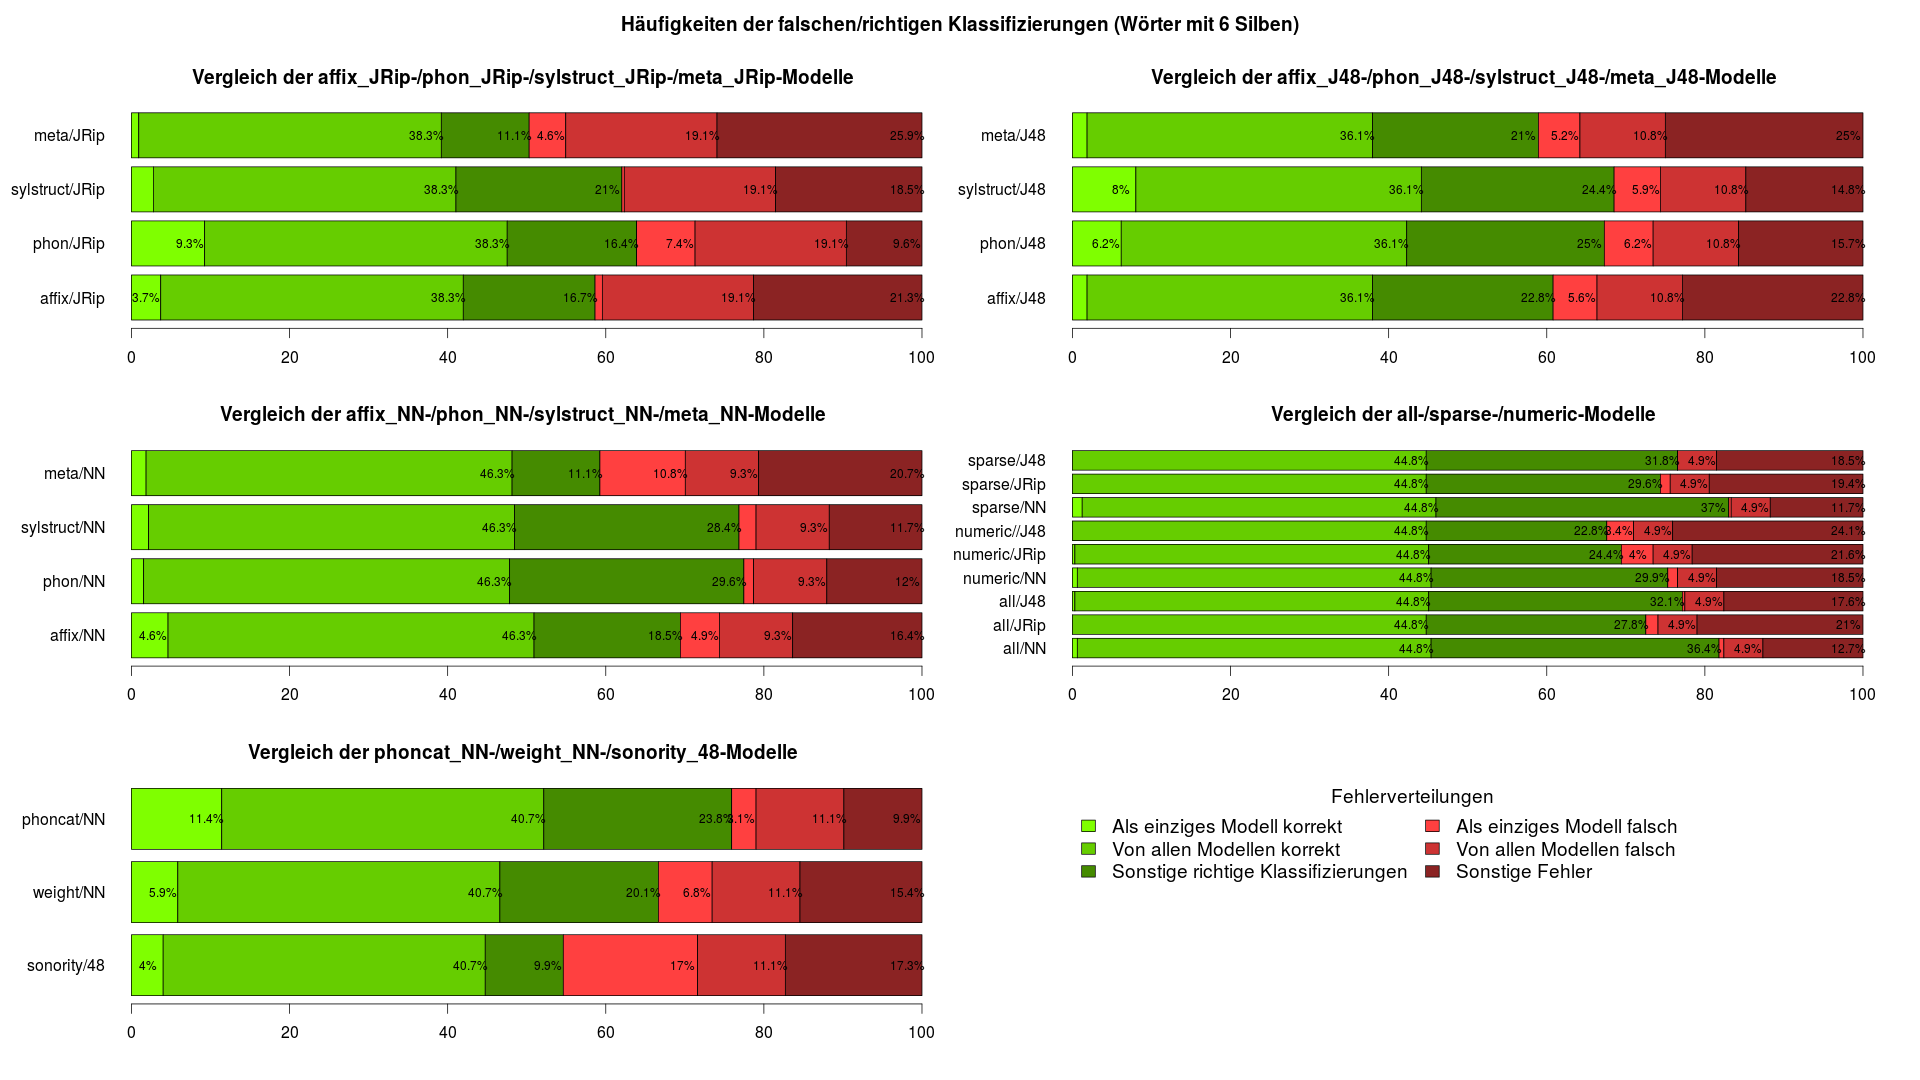
\includegraphics[width=22cm]{figures/compare/6syl.png}}\end{center}
%\begin{center}{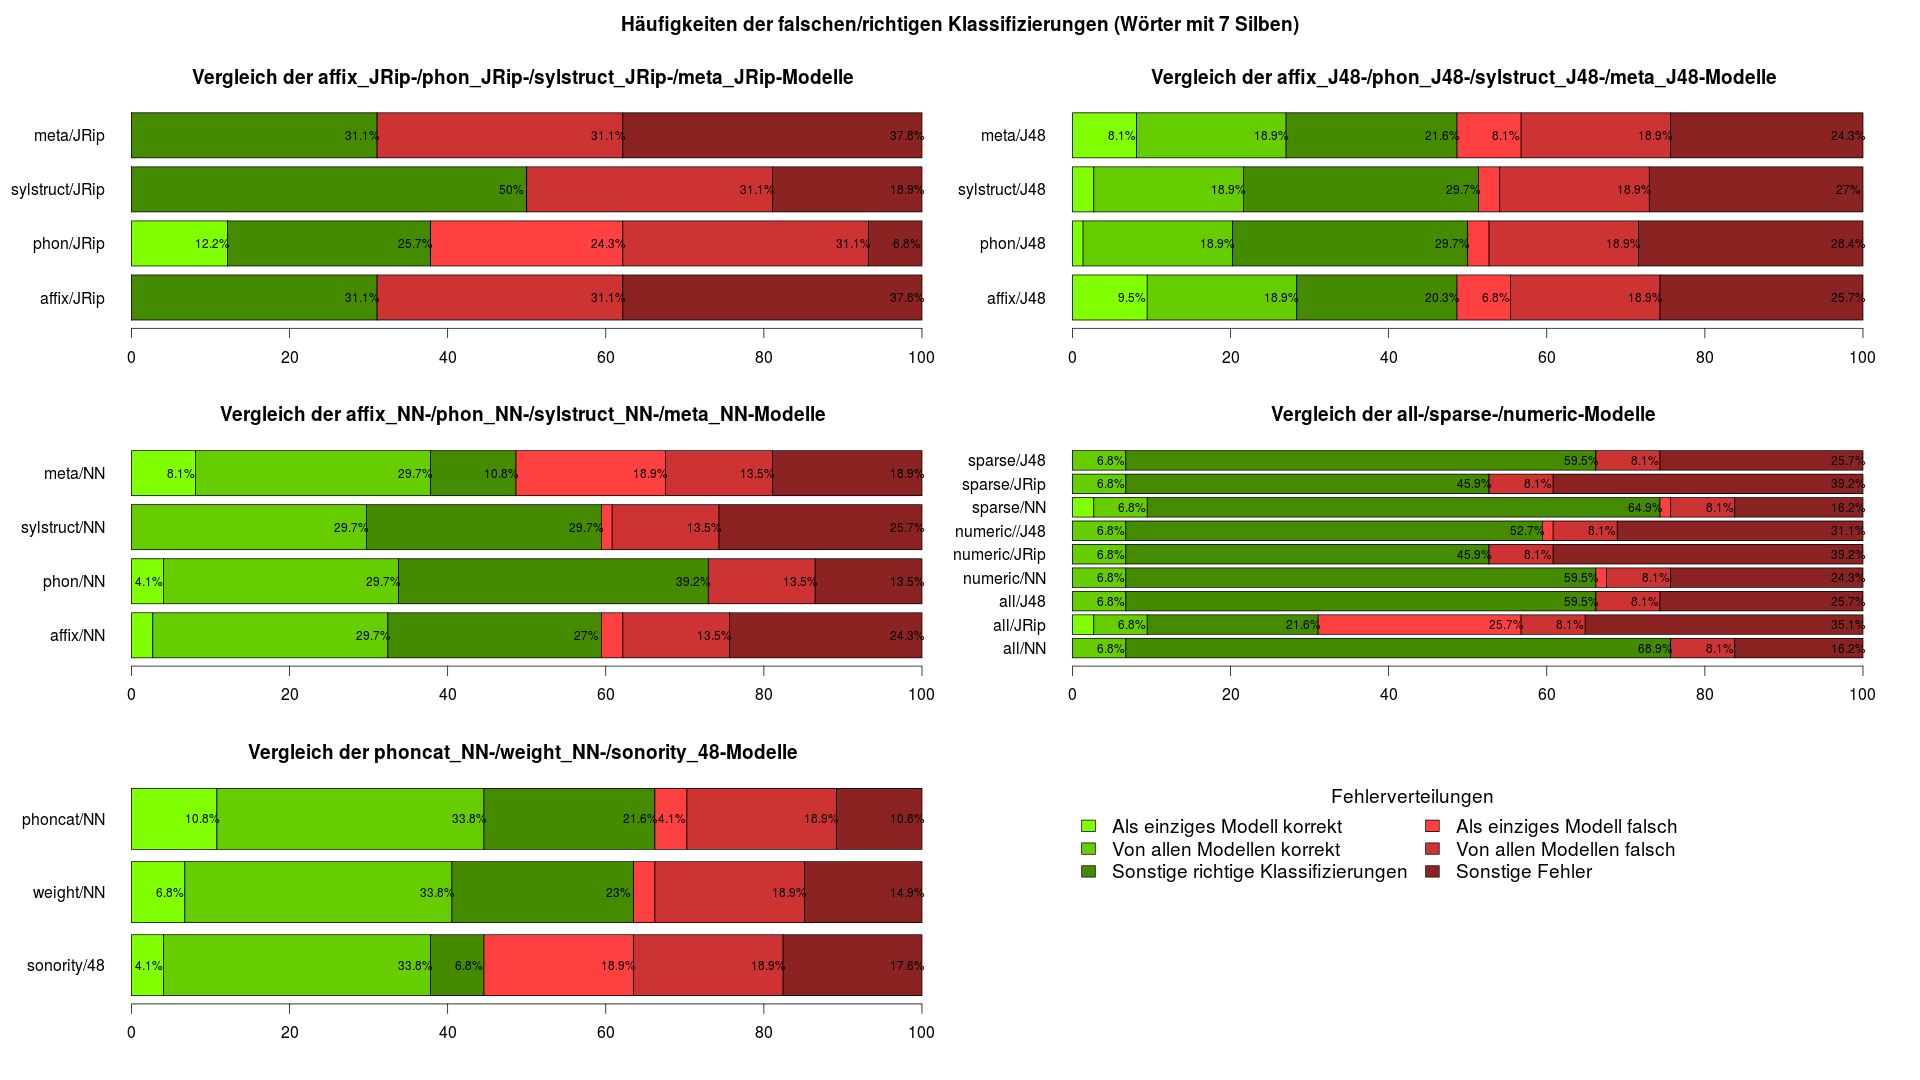
\includegraphics[width=22cm]{figures/compare/7syl.png}}\end{center}
%\end{landscape}

%\cleardoublepage